\documentclass[11pt,spanish]{article} % Idioma
\usepackage{babel}
\usepackage[T1]{fontenc}
\usepackage{textcomp, verbatim}
\usepackage[utf8]{inputenc} % Puede depender del instrucción, sistema o editor
\usepackage{wrapfig} % Imagenes
% \graphicspath{ {./imagenes/} }

\usepackage[left=2.75cm,top=2.5cm,right=2cm,bottom=2.5cm]{geometry} % Márgenes
%\usepackage{pstricks} % Gráficas, movilidad, árboles y otros

\usepackage{amssymb, amsmath} % Símbolos matemáticos
\usepackage{amsthm} % Teoremas, lemas, pruebas...
\usepackage{cancel} % Cancelar expresiones
\usepackage{multirow} % Tablas
\usepackage{multicol}

\usepackage{graphicx, float} % Inserción de imágenes
\usepackage{gnuplot-lua-tikz}
\usepackage{xcolor} % Colores
\usepackage{color}
\definecolor{gray97}{gray}{.97}
\definecolor{gray75}{gray}{.75}
\definecolor{gray45}{gray}{.45}

\usepackage[hidelinks]{hyperref}  % Enlaces
\usepackage{multirow} % Tablas
\usepackage{pgfplotstable}

\usepackage{listings} % Escribir código en diferentes lenguajes de programación
\usepackage{longtable} % para tablas largas
\lstset{ frame=Ltb,
framerule=0pt,
aboveskip=0.5cm,
framextopmargin=3pt,
framexbottommargin=3pt,
framexleftmargin=0.4cm,
framesep=0pt,
rulesep=.4pt,
backgroundcolor=\color{gray97},
rulesepcolor=\color{black},
%
stringstyle=\ttfamily,
showstringspaces = false,
basicstyle=\small\ttfamily,
commentstyle=\color{gray45},
keywordstyle=\bfseries,
%
numbers=left,
numbersep=15pt,
numberstyle=\tiny,
numberfirstline = false,
breaklines=true,
}


\title{Memoria de divide y vencerás}
\author{Rubén Morales Pérez
		\and Francisco Javier Morales Piqueras
		\and Bruno Santindrian Manzanedo
		\and Ignacio de Loyola Barragan Lozano
		\and Francisco Leopoldo Gallego Salido}
\date{\today}


% % % % % % % % % % % % % % % % % % % % % % % % % % % % % % % % %
%					 Inicio del documento
% % % % % % % % % % % % % % % % % % % % % % % % % % % % % % % % %
\begin{document}
\maketitle
\tableofcontents % Generando el indice
\newpage
\setlength\parindent{0pt} % Quitamos la sangría

%%%%%%%%%%%%%%%%%%%%%%%%%%%%%%%%%%%%%%%%%%%%%%%%%%%%%%%%%%%%%%%%%%%%%%%%%%%%%%%%%%
\section{Ejercicio 2}
\subsection{Enunciado del problema}
\textbf{Minimizando el número de visitas al proveedor:}\\

Un granjero necesita disponer siempre de un determinado fertilizante. La cantidad máxima que puede almacenar la consume en r días, y antes de que eso ocurra necesita acudir a una tienda del pueblo para abastecerse. El problema es que dicha tienda tiene un horario de apertura muy irregular (solo abre determinados días). El granjero conoce los días en que abre la tienda, y desea minimizar el número de desplazamientos al pueblo para abastecerse.\\

\begin{itemize}
\item Diseñar un algoritmo greedy que determine en qué días debe acudir al pueblo a comprar fertilizante durante un periodo de tiempo determinado (por ejemplo durante el siguiente mes).\\
\item Demostrar que el algoritmo encuentra siempre la solución  óptima.\\
\end{itemize}


\subsection{Diseño del algoritmo}

El algoritmo, al basarse en la filosofía greedy, intenta escoger la mejor solución en cada fase. En nuestro caso, la mejor solución pasa por ir a comprar el día más lejano posible que cumpla estas dos condiciones.\\
\begin{enumerate}
\item Que diste menos de r días de la ultima reposición.\\
\item Que la tienda esté abierta.\\
\end{enumerate}

\textbf{Ejemplo:}\\

\definecolor{cffffff}{RGB}{255,255,255}
\definecolor{cfcbb06}{RGB}{252,187,6} %naranja
\definecolor{c787878}{RGB}{120,120,120}
\definecolor{cff4040}{RGB}{255,64,64}
\definecolor{c409f40}{RGB}{64,159,64}


\begin{tikzpicture}[y=0.80pt, x=0.80pt, yscale=-3.400000, xscale=3.400000, inner sep=0pt, outer sep=0pt]
  \path[color=black,fill=cffffff,line join=miter,line cap=round,miter
          limit=4.00,even odd rule,line width=0.621pt,rounded corners=0.0000cm]
          (-10.0427,-12.5075) rectangle (180.1040,149.1172);
        \path[color=black,fill=c409f40,line join=miter,line cap=round,miter
          limit=4.00,even odd rule,line width=0.621pt,rounded corners=0.0000cm]
          (-9.9362,-12.4405) rectangle (180.2669,8.8984);
        \path[shift={(-0.36339,-16)},fill=cffffff] (0.0000,22.0472) node[above
          right] (text4254) {{\color{white}Lun}};
        \path[shift={(-0.36339,-16)},fill=cffffff] (28.3465,22.0472) node[above
          right] (text4256) {{\color{white}Mar}};
        \path[shift={(-0.36339,-16)},fill=cffffff] (56.6929,22.0472) node[above
          right] (text4258) {{\color{white}Mier}};
        \path[shift={(-0.36339,-16)},fill=cffffff] (85.0394,22.0472) node[above
          right] (text4260) {{\color{white}Jue}};
        \path[shift={(-0.36339,-16)},fill=cffffff] (113.3858,22.0472) node[above
          right] (text4262) {{\color{white}Vie}};
        \path[shift={(-0.36339,-16)},fill=cffffff] (141.7323,22.0472) node[above
          right] (text4264) {{\color{white}Sab}};
        \path[shift={(-0.36339,-16)},fill=cffffff] (170.0787,22.0472) node[above
          right] (text4266) {{\color{white}Dom}};
  \begin{scope}[shift={(-0.36339,-16)}]
    \path[fill=black] (0.0000,44.0945) node[above right] (text4270) {1};
    \path[fill=cfcbb06] (28.3465,44.0945) node[above right] (text4272) {{\color{cfcbb06}2}};
    \path[fill=cfcbb06] (56.6929,44.0945) node[above right] (text4274) {{\color{cfcbb06}3}};
    \path[fill=black] (85.0394,44.0945) node[above right] (text4276) {4};
    \path[fill=black] (113.3858,44.0945) node[above right] (text4278) {5};
    \path[fill=cfcbb06] (141.7323,44.0945) node[above right] (text4280) {{\color{cfcbb06}6}};
    \path[fill=black] (170.0787,44.0945) node[above right] (text4282) {7};
    \path[fill=black] (0.0000,66.1417) node[above right] (text4284) {8};
    \path[fill=black] (28.3465,66.1417) node[above right] (text4286) {9};
    \path[fill=cfcbb06] (56.6929,66.1417) node[above right] (text4288) {{\color{cfcbb06}10}};
    \path[fill=black] (85.0394,66.1417) node[above right] (text4290) {11};
    \path[fill=cfcbb06] (113.3858,66.1417) node[above right] (text4292) {{\color{cfcbb06}12}};
    \path[fill=cfcbb06] (141.7323,66.1417) node[above right] (text4294) {{\color{cfcbb06}13}};
    \path[fill=black] (170.0787,66.1417) node[above right] (text4296) {14};
    \path[fill=black] (0.0000,88.1890) node[above right] (text4298) {15};
    \path[fill=black] (28.3465,88.1890) node[above right] (text4300) {16};
    \path[fill=cfcbb06] (56.6929,88.1890) node[above right] (text4302) {{\color{cfcbb06}17}};
    \path[fill=black] (85.0394,88.1890) node[above right] (text4304) {18};
    \path[fill=black] (113.3858,88.1890) node[above right] (text4306) {19};
    \path[fill=cfcbb06] (141.7323,88.1890) node[above right] (text4308) {{\color{cfcbb06}20}};
    \path[fill=cfcbb06] (170.0787,88.1890) node[above right] (text4310) {{\color{cfcbb06}21}};
    \path[fill=black] (0.0000,110.2362) node[above right] (text4312) {22};
    \path[fill=black] (28.3465,110.2362) node[above right] (text4314) {23};
    \path[fill=cfcbb06] (56.6929,110.2362) node[above right] (text4316) {{\color{cfcbb06}24}};
    \path[fill=cfcbb06] (85.0394,110.2362) node[above right] (text4318) {{\color{cfcbb06}25}};
    \path[fill=black] (113.3858,110.2362) node[above right] (text4320) {26};
    \path[fill=cfcbb06] (141.7323,110.2362) node[above right] (text4322) {{\color{cfcbb06}27}};
    \path[fill=black] (170.0787,110.2362) node[above right] (text4324) {28};
    \path[fill=black] (0.0000,132.2835) node[above right] (text4326) {29};
    \path[fill=black] (28.3465,132.2835) node[above right] (text4328) {30};
    \path[color=black,draw=c787878,line join=miter,line cap=round,miter
      limit=4.00,even odd rule,line width=0.203pt,rounded corners=0.0000cm]
      (-7.6806,30.9845) rectangle (94.2501,46.7919);
    \path[color=black,draw=c787878,line join=miter,line cap=round,miter
      limit=4.00,even odd rule,line width=0.203pt,rounded corners=0.0000cm]
      (75.8081,31.0754) rectangle (177.7388,46.8828);
    \path[color=black,draw=c787878,line join=miter,line cap=round,miter
      limit=4.00,even odd rule,line width=0.199pt,rounded corners=0.0000cm]
      (161.6961,31.2035) rectangle (177.6106,46.7547);
    \path[color=black,draw=c787878,line join=miter,line cap=round,miter
      limit=4.00,even odd rule,line width=0.203pt,rounded corners=0.0000cm]
      (-8.0022,53.3748) rectangle (69.3161,69.2802);
    \path[color=black,draw=c787878,line join=miter,line cap=round,miter
      limit=4.00,even odd rule,line width=0.203pt,rounded corners=0.0000cm]
      (75.6277,53.6068) rectangle (178.2825,69.4116);
    \path[color=black,draw=c787878,line join=miter,line cap=round,miter
      limit=4.00,even odd rule,line width=0.199pt,rounded corners=0.0000cm]
      (161.1561,53.7388) rectangle (178.1506,69.2797);
    \path[color=black,draw=c787878,line join=miter,line cap=round,miter
      limit=4.00,even odd rule,line width=0.203pt,rounded corners=0.0000cm]
      (-8.0022,75.3598) rectangle (69.3161,91.2653);
    \path[color=black,draw=c787878,line join=miter,line cap=round,miter
      limit=4.00,even odd rule,line width=0.203pt,rounded corners=0.0000cm]
      (75.9898,75.7722) rectangle (177.9204,91.5797);
    \path[color=black,draw=c787878,line join=miter,line cap=round,miter
      limit=4.00,even odd rule,line width=0.203pt,rounded corners=0.0000cm]
      (-8.3165,97.7573) rectangle (93.6141,113.5647);
    \path[color=black,draw=c787878,line join=miter,line cap=round,miter
      limit=4.00,even odd rule,line width=0.203pt,rounded corners=0.0000cm]
      (102.1040,97.7075) rectangle (179.0604,113.6145);
    \path[color=black,draw=c787878,line join=miter,line cap=round,miter
      limit=4.00,even odd rule,line width=0.203pt,rounded corners=0.0000cm]
      (-8.7222,119.5184) rectangle (8.9867,135.7737);
    \path[draw=cff4040,line join=round,line cap=round,miter limit=4.00,nonzero
      rule,line width=0.305pt] (56.5484,39.0699) circle (0.2692cm);
    \path[draw=cff4040,line join=round,line cap=round,miter limit=4.00,nonzero
      rule,line width=0.305pt] (141.6724,39.1608) circle (0.2692cm);
    \path[draw=cff4040,line join=round,line cap=round,miter limit=4.00,nonzero
      rule,line width=0.305pt] (57.0027,61.1458) circle (0.2692cm);
    \path[draw=cff4040,line join=round,line cap=round,miter limit=4.00,nonzero
      rule,line width=0.305pt] (141.8541,61.1458) circle (0.2692cm);
    \path[draw=cff4040,line join=round,line cap=round,miter limit=4.00,nonzero
      rule,line width=0.305pt] (56.6393,83.4943) circle (0.2692cm);
    \path[draw=cff4040,line join=round,line cap=round,miter limit=4.00,nonzero
      rule,line width=0.305pt] (169.6533,83.4943) circle (0.2692cm);
    \path[draw=cff4040,line join=round,line cap=round,miter limit=4.00,nonzero
      rule,line width=0.305pt] (84.9836,105.6610) circle (0.2692cm);
    \path[draw=cff4040,line join=round,line cap=round,miter limit=4.00,nonzero
      rule,line width=0.305pt] (141.4907,105.8427) circle (0.2692cm);
  \end{scope}
  \path[color=black,fill=c409f40,line join=miter,line cap=round,miter
    limit=4.00,even odd rule,line width=0.621pt,rounded corners=0.0000cm]
    (-10.0426,125.4589) rectangle (180.1605,127.4576);
  \path[color=black,fill=c409f40,line join=miter,line cap=round,miter
    limit=4.00,even odd rule,line width=0.621pt,rounded corners=0.0000cm]
    (-10.0427,134.9070) rectangle (180.1605,139.6311);
  \path[color=black,fill=c787878,line join=miter,line cap=round,miter
    limit=4.00,even odd rule,line width=0.621pt,rounded corners=0.0000cm]
    (-4.5918,128.8) rectangle (-0.0494,133.0901);
  \path[color=black,fill=cfcbb06,line join=miter,line cap=round,miter
    limit=4.00,even odd rule,line width=0.621pt,rounded corners=0.0000cm]
    (59.8189,128.8) rectangle (64.3613,133.0901);
  \path[color=black,fill=cff4040,line join=miter,line cap=round,miter
    limit=4.00,even odd rule,line width=0.621pt,rounded corners=0.0000cm]
    (123.7755,128.8) rectangle (128.3178,133.1809);
  \path[fill=black,line join=miter,line cap=butt,line width=0.800pt]
    (1.9492,133) node[above right] (text6322) {Reserva (4 días)};
  \path[fill=black,line join=miter,line cap=butt,line width=0.800pt]
    (66.6529,133) node[above right] (text6322-2) {Tienda abierta};
  \path[fill=black,line join=miter,line cap=butt,line width=0.800pt]
    (130.3368,133) node[above right] (text6322-4) {Visita};

\end{tikzpicture}



\subsubsection{Representación del algoritmo}

Para programar el problema lo hemos modelado de la siguiente manera:\\

\begin{itemize}
\item Un vector de booleanos representa los días que abre la tienda.\\
Por ejemplo [1, 0, 0, 1, 0, 1] significa que la tienda abre los días 1, 4 y 6.\\
\item Una lista de enteros almacena los días que el granjero tiene que ir a comprar.
\end{itemize}


\subsubsection{Implementación del algoritmo}

La implementación se encuentra en \textit{minimizar\_visitas.cpp}.\\
La función clave es \textbf{minimize\_visits()}, en la que, para buscar el día mas lejano posible, se accede a la posición i+r del vector y se recorre hacia atrás hasta que se encuentra un día en el que la tienda esté abierta.\\

También hemos implementado otro algoritmo con el fin de hacer comparaciones, en el que el día de visita se elige aleatoriamente en el rango [i, i+r-1]. Esta implementación se encuentra en \textit{visitas\_aleatorias.cpp}\\



\subsection{Demostración de la optimalidad}

Sean:\\
\begin{itemize}
\item \textbf{p} la duración del periodo (ej: 30 días)
\item \textbf{r} la duración de la reserva
\item \textbf{a} vector de tamaño p que representa los días que abre la tienda\\
La tienda abre el día $n$ si $a_n = 1$\\
La tienda no abre el día $n$ si $a_n = 0$
\item \textbf{d} el vector que almacena los días de visita\\
$d_{i+1} = d_i + k_i\ /\ k_i \in \{x \in \mathbb{N} : 0<x<r\ y\ a_{d_i+x} = 1\}$\\
\end{itemize}

Formulamos dos ecuaciones:\\

$d_{i+1}^h = d_i^h + h_i$ donde $h_i = max\{x \in \mathbb{N} : 0<x<r\ y\ a_{d_i+x} = 1\}$\\
Podemos definir $n \in \mathbb{N}\ /\ d_n^h = min\{d_i^h: d_i^h + r > p\}$ como el índice del último día que necesitamos ir a comprar.\\

$d_{i+1}^t = d_i^t + t_i$ donde $t_i \in \{x \in \mathbb{N} : 0<x<r\ y\ a_{d_i+x} = 1\}\ /\ t_i < h_i$ para algún $i<n$\\

$d^{h}$ representa la aproximación greedy, mientras que $d^{t}$ representa cualquier otro algoritmo.\\

Por las definiciones anteriores sabemos que $\exists m \in \mathbb{N}\ /\ d_i^{t} \leq d_i^{h}\ \forall i,\ m \leq i<n \Rightarrow d_n^{t} \leq d_n^{h}$\\
Distinguimos dos casos:\\
\begin{enumerate}
\item Si $p-r < d_n^{t} \leq d_n^{h}$ las dos opciones son igual de buenas\\
\item Si $d_n^{t} < p-r < d_n^{h}$ la opción greedy es mejor\\
\end{enumerate}

De aquí deducimos que utilizar el enfoque greedy en este caso siempre nos da el mejor resultado.\\



\subsection{Resultados empíricos}
\subsubsection{Eficiencia}

Aunque en esta ocasión la eficiencia no es especialmente importante, está claro que el tiempo aumenta linealmente en relación al tamaño del periodo de tiempo O(p).\\

Además también aumenta al disminuir la duración de la reserva, tardando más con un periodo grande y una reserva pequeña.\\

\begin{center}
\resizebox{6in}{!}{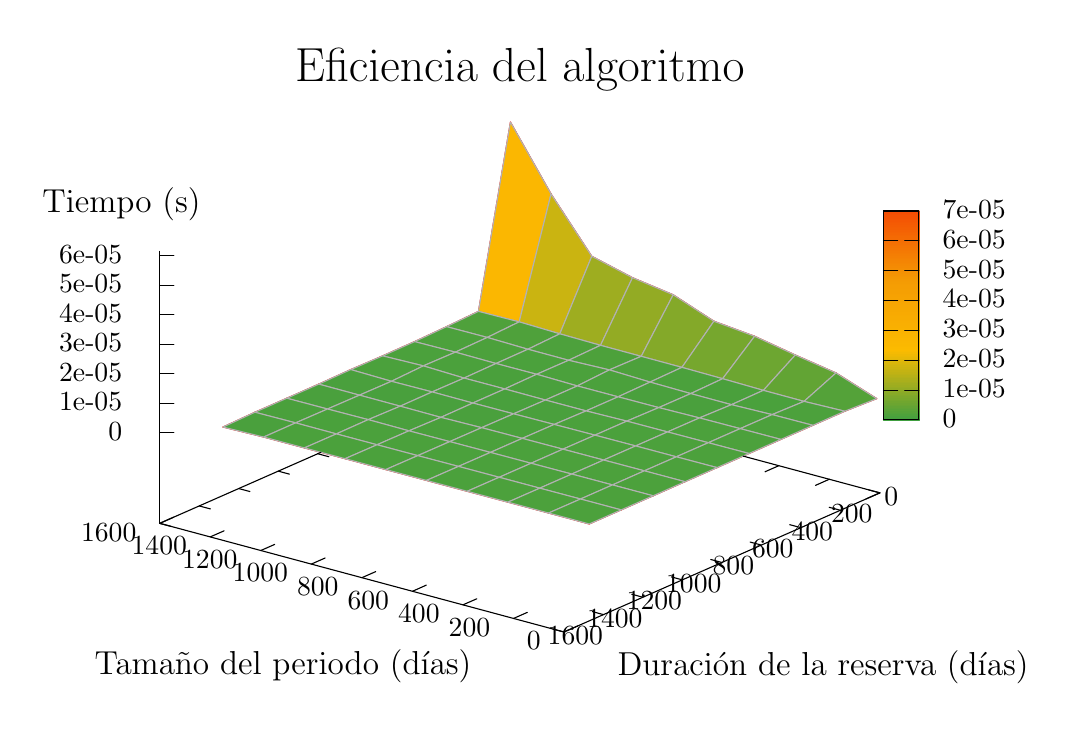
\begin{tikzpicture}[gnuplot]
%% generated with GNUPLOT 4.6p4 (Lua 5.1; terminal rev. 99, script rev. 100)
%% sáb 30 abr 2016 19:56:30 CEST
\path (0.000,0.000) rectangle (12.500,8.750);
\gpcolor{color=gp lt color border}
\node[gp node center,font={\fontsize{16pt}{19.2pt}\selectfont}] at (6.250,8.163) {Eficiencia del algoritmo};
\gpcolor{color=gp lt color 0}
\gpsetlinetype{gp lt plot 0}
\gpsetlinewidth{1.00}
\draw[gp path] (6.131,7.551)--(5.725,5.147);
\draw[gp path] (5.320,4.953)--(5.725,5.147);
\draw[gp path] (6.242,5.014)--(5.725,5.147);
\draw[gp path] (6.647,6.638)--(6.242,5.014);
\draw[gp path] (5.837,4.816)--(6.242,5.014);
\draw[gp path] (6.758,4.862)--(6.242,5.014);
\draw[gp path] (4.914,4.763)--(5.320,4.953);
\draw[gp path] (5.837,4.816)--(5.320,4.953);
\draw[gp path] (7.164,5.847)--(6.758,4.862);
\draw[gp path] (6.353,4.666)--(6.758,4.862);
\draw[gp path] (7.275,4.716)--(6.758,4.862);
\draw[gp path] (5.431,4.629)--(5.837,4.816);
\draw[gp path] (6.353,4.666)--(5.837,4.816);
\draw[gp path] (4.508,4.582)--(4.914,4.763);
\draw[gp path] (5.431,4.629)--(4.914,4.763);
\draw[gp path] (7.681,5.575)--(7.275,4.716);
\draw[gp path] (6.870,4.526)--(7.275,4.716);
\draw[gp path] (7.792,4.576)--(7.275,4.716);
\draw[gp path] (6.647,6.638)--(7.164,5.847);
\draw[gp path] (7.681,5.575)--(7.164,5.847);
\draw[gp path] (5.948,4.485)--(6.353,4.666);
\draw[gp path] (6.870,4.526)--(6.353,4.666);
\draw[gp path] (5.025,4.455)--(5.431,4.629);
\draw[gp path] (5.948,4.485)--(5.431,4.629);
\draw[gp path] (8.198,5.358)--(7.681,5.575);
\draw[gp path] (4.103,4.408)--(4.508,4.582);
\draw[gp path] (5.025,4.455)--(4.508,4.582);
\draw[gp path] (8.198,5.358)--(7.792,4.576);
\draw[gp path] (7.387,4.404)--(7.792,4.576);
\draw[gp path] (8.309,4.436)--(7.792,4.576);
\draw[gp path] (6.131,7.551)--(6.647,6.638);
\draw[gp path] (6.464,4.348)--(6.870,4.526);
\draw[gp path] (7.387,4.404)--(6.870,4.526);
\draw[gp path] (5.542,4.300)--(5.948,4.485);
\draw[gp path] (6.464,4.348)--(5.948,4.485);
\draw[gp path] (8.715,5.022)--(8.198,5.358);
\draw[gp path] (4.620,4.259)--(5.025,4.455);
\draw[gp path] (5.542,4.300)--(5.025,4.455);
\draw[gp path] (8.309,4.436)--(8.715,5.022);
\draw[gp path] (9.232,4.831)--(8.715,5.022);
\draw[gp path] (7.904,4.249)--(8.309,4.436);
\draw[gp path] (8.826,4.292)--(8.309,4.436);
\draw[gp path] (3.697,4.223)--(4.103,4.408);
\draw[gp path] (4.620,4.259)--(4.103,4.408);
\draw[gp path] (6.981,4.200)--(7.387,4.404);
\draw[gp path] (7.904,4.249)--(7.387,4.404);
\draw[gp path] (6.059,4.162)--(6.464,4.348);
\draw[gp path] (6.981,4.200)--(6.464,4.348);
\draw[gp path] (8.826,4.292)--(9.232,4.831);
\draw[gp path] (9.749,4.593)--(9.232,4.831);
\draw[gp path] (5.137,4.124)--(5.542,4.300);
\draw[gp path] (6.059,4.162)--(5.542,4.300);
\draw[gp path] (8.421,4.103)--(8.826,4.292);
\draw[gp path] (9.343,4.144)--(8.826,4.292);
\draw[gp path] (4.214,4.083)--(4.620,4.259);
\draw[gp path] (5.137,4.124)--(4.620,4.259);
\draw[gp path] (7.498,4.062)--(7.904,4.249);
\draw[gp path] (8.421,4.103)--(7.904,4.249);
\draw[gp path] (3.291,4.044)--(3.697,4.223);
\draw[gp path] (4.214,4.083)--(3.697,4.223);
\draw[gp path] (9.343,4.144)--(9.749,4.593);
\draw[gp path] (10.266,4.365)--(9.749,4.593);
\draw[gp path] (6.575,4.021)--(6.981,4.200);
\draw[gp path] (7.498,4.062)--(6.981,4.200);
\draw[gp path] (5.654,3.983)--(6.059,4.162);
\draw[gp path] (6.575,4.021)--(6.059,4.162);
\draw[gp path] (8.938,3.962)--(9.343,4.144);
\draw[gp path] (9.860,4.004)--(9.343,4.144);
\draw[gp path] (4.731,3.943)--(5.137,4.124);
\draw[gp path] (5.654,3.983)--(5.137,4.124);
\draw[gp path] (9.860,4.004)--(10.266,4.365);
\draw[gp path] (10.783,4.039)--(10.266,4.365);
\draw[gp path] (8.015,3.925)--(8.421,4.103);
\draw[gp path] (8.938,3.962)--(8.421,4.103);
\draw[gp path] (3.808,3.907)--(4.214,4.083);
\draw[gp path] (4.731,3.943)--(4.214,4.083);
\draw[gp path] (7.092,3.883)--(7.498,4.062);
\draw[gp path] (8.015,3.925)--(7.498,4.062);
\draw[gp path] (10.377,3.879)--(10.783,4.039);
\draw[gp path] (2.886,3.866)--(3.291,4.044);
\draw[gp path] (3.808,3.907)--(3.291,4.044);
\draw[gp path] (6.171,3.846)--(6.575,4.021);
\draw[gp path] (7.092,3.883)--(6.575,4.021);
\draw[gp path] (9.455,3.836)--(9.860,4.004);
\draw[gp path] (10.377,3.879)--(9.860,4.004);
\draw[gp path] (5.248,3.801)--(5.654,3.983);
\draw[gp path] (6.171,3.846)--(5.654,3.983);
\draw[gp path] (8.532,3.794)--(8.938,3.962);
\draw[gp path] (9.455,3.836)--(8.938,3.962);
\draw[gp path] (4.325,3.772)--(4.731,3.943);
\draw[gp path] (5.248,3.801)--(4.731,3.943);
\draw[gp path] (7.609,3.753)--(8.015,3.925);
\draw[gp path] (8.532,3.794)--(8.015,3.925);
\draw[gp path] (3.403,3.731)--(3.808,3.907);
\draw[gp path] (4.325,3.772)--(3.808,3.907);
\draw[gp path] (6.687,3.711)--(7.092,3.883);
\draw[gp path] (7.609,3.753)--(7.092,3.883);
\draw[gp path] (2.480,3.678)--(2.886,3.866);
\draw[gp path] (3.403,3.731)--(2.886,3.866);
\draw[gp path] (9.972,3.700)--(10.377,3.879);
\draw[gp path] (5.765,3.670)--(6.171,3.846);
\draw[gp path] (6.687,3.711)--(6.171,3.846);
\draw[gp path] (9.049,3.658)--(9.455,3.836);
\draw[gp path] (9.972,3.700)--(9.455,3.836);
\draw[gp path] (4.842,3.630)--(5.248,3.801);
\draw[gp path] (5.765,3.670)--(5.248,3.801);
\draw[gp path] (8.126,3.616)--(8.532,3.794);
\draw[gp path] (9.049,3.658)--(8.532,3.794);
\draw[gp path] (3.920,3.591)--(4.325,3.772);
\draw[gp path] (4.842,3.630)--(4.325,3.772);
\draw[gp path] (7.204,3.575)--(7.609,3.753);
\draw[gp path] (8.126,3.616)--(7.609,3.753);
\draw[gp path] (2.997,3.551)--(3.403,3.731);
\draw[gp path] (3.920,3.591)--(3.403,3.731);
\draw[gp path] (6.281,3.534)--(6.687,3.711);
\draw[gp path] (7.204,3.575)--(6.687,3.711);
\draw[gp path] (2.997,3.551)--(2.480,3.678);
\draw[gp path] (9.566,3.521)--(9.972,3.700);
\draw[gp path] (5.360,3.493)--(5.765,3.670);
\draw[gp path] (6.281,3.534)--(5.765,3.670);
\draw[gp path] (8.644,3.479)--(9.049,3.658);
\draw[gp path] (9.566,3.521)--(9.049,3.658);
\draw[gp path] (4.437,3.453)--(4.842,3.630);
\draw[gp path] (5.360,3.493)--(4.842,3.630);
\draw[gp path] (7.721,3.438)--(8.126,3.616);
\draw[gp path] (8.644,3.479)--(8.126,3.616);
\draw[gp path] (3.514,3.413)--(3.920,3.591);
\draw[gp path] (4.437,3.453)--(3.920,3.591);
\draw[gp path] (6.798,3.397)--(7.204,3.575);
\draw[gp path] (7.721,3.438)--(7.204,3.575);
\draw[gp path] (3.514,3.413)--(2.997,3.551);
\draw[gp path] (5.877,3.356)--(6.281,3.534);
\draw[gp path] (6.798,3.397)--(6.281,3.534);
\draw[gp path] (9.161,3.342)--(9.566,3.521);
\draw[gp path] (4.954,3.315)--(5.360,3.493);
\draw[gp path] (5.877,3.356)--(5.360,3.493);
\draw[gp path] (8.238,3.300)--(8.644,3.479);
\draw[gp path] (9.161,3.342)--(8.644,3.479);
\draw[gp path] (4.031,3.276)--(4.437,3.453);
\draw[gp path] (4.954,3.315)--(4.437,3.453);
\draw[gp path] (7.315,3.259)--(7.721,3.438);
\draw[gp path] (8.238,3.300)--(7.721,3.438);
\draw[gp path] (4.031,3.276)--(3.514,3.413);
\draw[gp path] (6.393,3.218)--(6.798,3.397);
\draw[gp path] (7.315,3.259)--(6.798,3.397);
\draw[gp path] (5.471,3.178)--(5.877,3.356);
\draw[gp path] (6.393,3.218)--(5.877,3.356);
\draw[gp path] (8.755,3.163)--(9.161,3.342);
\draw[gp path] (4.548,3.138)--(4.954,3.315);
\draw[gp path] (5.471,3.178)--(4.954,3.315);
\draw[gp path] (7.832,3.122)--(8.238,3.300);
\draw[gp path] (8.755,3.163)--(8.238,3.300);
\draw[gp path] (4.548,3.138)--(4.031,3.276);
\draw[gp path] (6.910,3.081)--(7.315,3.259);
\draw[gp path] (7.832,3.122)--(7.315,3.259);
\draw[gp path] (5.988,3.040)--(6.393,3.218);
\draw[gp path] (6.910,3.081)--(6.393,3.218);
\draw[gp path] (5.065,3.000)--(5.471,3.178);
\draw[gp path] (5.988,3.040)--(5.471,3.178);
\draw[gp path] (8.349,2.984)--(8.755,3.163);
\draw[gp path] (5.065,3.000)--(4.548,3.138);
\draw[gp path] (7.427,2.943)--(7.832,3.122);
\draw[gp path] (8.349,2.984)--(7.832,3.122);
\draw[gp path] (6.504,2.902)--(6.910,3.081);
\draw[gp path] (7.427,2.943)--(6.910,3.081);
\draw[gp path] (5.582,2.862)--(5.988,3.040);
\draw[gp path] (6.504,2.902)--(5.988,3.040);
\draw[gp path] (5.582,2.862)--(5.065,3.000);
\draw[gp path] (7.944,2.805)--(8.349,2.984);
\draw[gp path] (7.021,2.764)--(7.427,2.943);
\draw[gp path] (7.944,2.805)--(7.427,2.943);
\draw[gp path] (6.099,2.724)--(6.504,2.902);
\draw[gp path] (7.021,2.764)--(6.504,2.902);
\draw[gp path] (6.099,2.724)--(5.582,2.862);
\draw[gp path] (7.538,2.626)--(7.944,2.805);
\draw[gp path] (6.615,2.586)--(7.021,2.764);
\draw[gp path] (7.538,2.626)--(7.021,2.764);
\draw[gp path] (6.615,2.586)--(6.099,2.724);
\draw[gp path] (7.132,2.447)--(7.538,2.626);
\draw[gp path] (7.132,2.447)--(6.615,2.586);
\gpfill{rgb color={0.984,0.716,0.002}} (6.131,7.551)--(6.647,6.638)--(6.242,5.014)--(5.725,5.147)--cycle;
\gpcolor{color=gp lt color axes}
\gpsetlinetype{gp lt plot 3}
\draw[gp path] (6.131,7.551)--(5.725,5.147)--(6.242,5.014)--(6.647,6.638)--cycle;
\gpfill{rgb color={0.311,0.632,0.231}} (5.725,5.147)--(6.242,5.014)--(5.837,4.816)--(5.320,4.953)--cycle;
\draw[gp path] (5.725,5.147)--(5.320,4.953)--(5.837,4.816)--(6.242,5.014)--cycle;
\gpfill{rgb color={0.300,0.631,0.234}} (5.320,4.953)--(5.837,4.816)--(5.431,4.629)--(4.914,4.763)--cycle;
\draw[gp path] (5.320,4.953)--(4.914,4.763)--(5.431,4.629)--(5.837,4.816)--cycle;
\gpfill{rgb color={0.296,0.630,0.236}} (4.914,4.763)--(5.431,4.629)--(5.025,4.455)--(4.508,4.582)--cycle;
\draw[gp path] (4.914,4.763)--(4.508,4.582)--(5.025,4.455)--(5.431,4.629)--cycle;
\gpfill{rgb color={0.294,0.630,0.236}} (4.508,4.582)--(5.025,4.455)--(4.620,4.259)--(4.103,4.408)--cycle;
\draw[gp path] (4.508,4.582)--(4.103,4.408)--(4.620,4.259)--(5.025,4.455)--cycle;
\gpfill{rgb color={0.290,0.629,0.238}} (4.103,4.408)--(4.620,4.259)--(4.214,4.083)--(3.697,4.223)--cycle;
\draw[gp path] (4.103,4.408)--(3.697,4.223)--(4.214,4.083)--(4.620,4.259)--cycle;
\gpfill{rgb color={0.289,0.629,0.238}} (3.697,4.223)--(4.214,4.083)--(3.808,3.907)--(3.291,4.044)--cycle;
\draw[gp path] (3.697,4.223)--(3.291,4.044)--(3.808,3.907)--(4.214,4.083)--cycle;
\gpfill{rgb color={0.291,0.629,0.237}} (3.291,4.044)--(3.808,3.907)--(3.403,3.731)--(2.886,3.866)--cycle;
\draw[gp path] (3.291,4.044)--(2.886,3.866)--(3.403,3.731)--(3.808,3.907)--cycle;
\gpfill{rgb color={0.289,0.629,0.238}} (2.886,3.866)--(3.403,3.731)--(2.997,3.551)--(2.480,3.678)--cycle;
\draw[gp path] (2.886,3.866)--(2.480,3.678)--(2.997,3.551)--(3.403,3.731)--cycle;
\gpfill{rgb color={0.791,0.704,0.067}} (6.647,6.638)--(7.164,5.847)--(6.758,4.862)--(6.242,5.014)--cycle;
\draw[gp path] (6.647,6.638)--(6.242,5.014)--(6.758,4.862)--(7.164,5.847)--cycle;
\gpfill{rgb color={0.308,0.632,0.232}} (6.242,5.014)--(6.758,4.862)--(6.353,4.666)--(5.837,4.816)--cycle;
\draw[gp path] (6.242,5.014)--(5.837,4.816)--(6.353,4.666)--(6.758,4.862)--cycle;
\gpfill{rgb color={0.298,0.631,0.235}} (5.837,4.816)--(6.353,4.666)--(5.948,4.485)--(5.431,4.629)--cycle;
\draw[gp path] (5.837,4.816)--(5.431,4.629)--(5.948,4.485)--(6.353,4.666)--cycle;
\gpfill{rgb color={0.295,0.630,0.236}} (5.431,4.629)--(5.948,4.485)--(5.542,4.300)--(5.025,4.455)--cycle;
\draw[gp path] (5.431,4.629)--(5.025,4.455)--(5.542,4.300)--(5.948,4.485)--cycle;
\gpfill{rgb color={0.291,0.630,0.237}} (5.025,4.455)--(5.542,4.300)--(5.137,4.124)--(4.620,4.259)--cycle;
\draw[gp path] (5.025,4.455)--(4.620,4.259)--(5.137,4.124)--(5.542,4.300)--cycle;
\gpfill{rgb color={0.288,0.629,0.238}} (4.620,4.259)--(5.137,4.124)--(4.731,3.943)--(4.214,4.083)--cycle;
\draw[gp path] (4.620,4.259)--(4.214,4.083)--(4.731,3.943)--(5.137,4.124)--cycle;
\gpfill{rgb color={0.290,0.629,0.238}} (4.214,4.083)--(4.731,3.943)--(4.325,3.772)--(3.808,3.907)--cycle;
\draw[gp path] (4.214,4.083)--(3.808,3.907)--(4.325,3.772)--(4.731,3.943)--cycle;
\gpfill{rgb color={0.292,0.630,0.237}} (3.808,3.907)--(4.325,3.772)--(3.920,3.591)--(3.403,3.731)--cycle;
\draw[gp path] (3.808,3.907)--(3.403,3.731)--(3.920,3.591)--(4.325,3.772)--cycle;
\gpfill{rgb color={0.293,0.630,0.237}} (3.403,3.731)--(3.920,3.591)--(3.514,3.413)--(2.997,3.551)--cycle;
\draw[gp path] (3.403,3.731)--(2.997,3.551)--(3.514,3.413)--(3.920,3.591)--cycle;
\gpfill{rgb color={0.621,0.679,0.125}} (7.164,5.847)--(7.681,5.575)--(7.275,4.716)--(6.758,4.862)--cycle;
\draw[gp path] (7.164,5.847)--(6.758,4.862)--(7.275,4.716)--(7.681,5.575)--cycle;
\gpfill{rgb color={0.301,0.631,0.234}} (6.758,4.862)--(7.275,4.716)--(6.870,4.526)--(6.353,4.666)--cycle;
\draw[gp path] (6.758,4.862)--(6.353,4.666)--(6.870,4.526)--(7.275,4.716)--cycle;
\gpfill{rgb color={0.295,0.630,0.236}} (6.353,4.666)--(6.870,4.526)--(6.464,4.348)--(5.948,4.485)--cycle;
\draw[gp path] (6.353,4.666)--(5.948,4.485)--(6.464,4.348)--(6.870,4.526)--cycle;
\gpfill{rgb color={0.291,0.629,0.237}} (5.948,4.485)--(6.464,4.348)--(6.059,4.162)--(5.542,4.300)--cycle;
\draw[gp path] (5.948,4.485)--(5.542,4.300)--(6.059,4.162)--(6.464,4.348)--cycle;
\gpfill{rgb color={0.288,0.629,0.238}} (5.542,4.300)--(6.059,4.162)--(5.654,3.983)--(5.137,4.124)--cycle;
\draw[gp path] (5.542,4.300)--(5.137,4.124)--(5.654,3.983)--(6.059,4.162)--cycle;
\gpfill{rgb color={0.288,0.629,0.238}} (5.137,4.124)--(5.654,3.983)--(5.248,3.801)--(4.731,3.943)--cycle;
\draw[gp path] (5.137,4.124)--(4.731,3.943)--(5.248,3.801)--(5.654,3.983)--cycle;
\gpfill{rgb color={0.290,0.629,0.238}} (4.731,3.943)--(5.248,3.801)--(4.842,3.630)--(4.325,3.772)--cycle;
\draw[gp path] (4.731,3.943)--(4.325,3.772)--(4.842,3.630)--(5.248,3.801)--cycle;
\gpfill{rgb color={0.293,0.630,0.237}} (4.325,3.772)--(4.842,3.630)--(4.437,3.453)--(3.920,3.591)--cycle;
\draw[gp path] (4.325,3.772)--(3.920,3.591)--(4.437,3.453)--(4.842,3.630)--cycle;
\gpfill{rgb color={0.293,0.630,0.237}} (3.920,3.591)--(4.437,3.453)--(4.031,3.276)--(3.514,3.413)--cycle;
\draw[gp path] (3.920,3.591)--(3.514,3.413)--(4.031,3.276)--(4.437,3.453)--cycle;
\gpfill{rgb color={0.575,0.672,0.141}} (7.681,5.575)--(8.198,5.358)--(7.792,4.576)--(7.275,4.716)--cycle;
\draw[gp path] (7.681,5.575)--(7.275,4.716)--(7.792,4.576)--(8.198,5.358)--cycle;
\gpfill{rgb color={0.303,0.631,0.233}} (7.275,4.716)--(7.792,4.576)--(7.387,4.404)--(6.870,4.526)--cycle;
\draw[gp path] (7.275,4.716)--(6.870,4.526)--(7.387,4.404)--(7.792,4.576)--cycle;
\gpfill{rgb color={0.296,0.630,0.236}} (6.870,4.526)--(7.387,4.404)--(6.981,4.200)--(6.464,4.348)--cycle;
\draw[gp path] (6.870,4.526)--(6.464,4.348)--(6.981,4.200)--(7.387,4.404)--cycle;
\gpfill{rgb color={0.289,0.629,0.238}} (6.464,4.348)--(6.981,4.200)--(6.575,4.021)--(6.059,4.162)--cycle;
\draw[gp path] (6.464,4.348)--(6.059,4.162)--(6.575,4.021)--(6.981,4.200)--cycle;
\gpfill{rgb color={0.288,0.629,0.238}} (6.059,4.162)--(6.575,4.021)--(6.171,3.846)--(5.654,3.983)--cycle;
\draw[gp path] (6.059,4.162)--(5.654,3.983)--(6.171,3.846)--(6.575,4.021)--cycle;
\gpfill{rgb color={0.289,0.629,0.238}} (5.654,3.983)--(6.171,3.846)--(5.765,3.670)--(5.248,3.801)--cycle;
\draw[gp path] (5.654,3.983)--(5.248,3.801)--(5.765,3.670)--(6.171,3.846)--cycle;
\gpfill{rgb color={0.291,0.629,0.237}} (5.248,3.801)--(5.765,3.670)--(5.360,3.493)--(4.842,3.630)--cycle;
\draw[gp path] (5.248,3.801)--(4.842,3.630)--(5.360,3.493)--(5.765,3.670)--cycle;
\gpfill{rgb color={0.293,0.630,0.237}} (4.842,3.630)--(5.360,3.493)--(4.954,3.315)--(4.437,3.453)--cycle;
\draw[gp path] (4.842,3.630)--(4.437,3.453)--(4.954,3.315)--(5.360,3.493)--cycle;
\gpfill{rgb color={0.294,0.630,0.236}} (4.437,3.453)--(4.954,3.315)--(4.548,3.138)--(4.031,3.276)--cycle;
\draw[gp path] (4.437,3.453)--(4.031,3.276)--(4.548,3.138)--(4.954,3.315)--cycle;
\gpfill{rgb color={0.516,0.663,0.161}} (8.198,5.358)--(8.715,5.022)--(8.309,4.436)--(7.792,4.576)--cycle;
\draw[gp path] (8.198,5.358)--(7.792,4.576)--(8.309,4.436)--(8.715,5.022)--cycle;
\gpfill{rgb color={0.302,0.631,0.234}} (7.792,4.576)--(8.309,4.436)--(7.904,4.249)--(7.387,4.404)--cycle;
\draw[gp path] (7.792,4.576)--(7.387,4.404)--(7.904,4.249)--(8.309,4.436)--cycle;
\gpfill{rgb color={0.294,0.630,0.236}} (7.387,4.404)--(7.904,4.249)--(7.498,4.062)--(6.981,4.200)--cycle;
\draw[gp path] (7.387,4.404)--(6.981,4.200)--(7.498,4.062)--(7.904,4.249)--cycle;
\gpfill{rgb color={0.287,0.629,0.239}} (6.981,4.200)--(7.498,4.062)--(7.092,3.883)--(6.575,4.021)--cycle;
\draw[gp path] (6.981,4.200)--(6.575,4.021)--(7.092,3.883)--(7.498,4.062)--cycle;
\gpfill{rgb color={0.289,0.629,0.238}} (6.575,4.021)--(7.092,3.883)--(6.687,3.711)--(6.171,3.846)--cycle;
\draw[gp path] (6.575,4.021)--(6.171,3.846)--(6.687,3.711)--(7.092,3.883)--cycle;
\gpfill{rgb color={0.292,0.630,0.237}} (6.171,3.846)--(6.687,3.711)--(6.281,3.534)--(5.765,3.670)--cycle;
\draw[gp path] (6.171,3.846)--(5.765,3.670)--(6.281,3.534)--(6.687,3.711)--cycle;
\gpfill{rgb color={0.294,0.630,0.236}} (5.765,3.670)--(6.281,3.534)--(5.877,3.356)--(5.360,3.493)--cycle;
\draw[gp path] (5.765,3.670)--(5.360,3.493)--(5.877,3.356)--(6.281,3.534)--cycle;
\gpfill{rgb color={0.295,0.630,0.236}} (5.360,3.493)--(5.877,3.356)--(5.471,3.178)--(4.954,3.315)--cycle;
\draw[gp path] (5.360,3.493)--(4.954,3.315)--(5.471,3.178)--(5.877,3.356)--cycle;
\gpfill{rgb color={0.295,0.630,0.236}} (4.954,3.315)--(5.471,3.178)--(5.065,3.000)--(4.548,3.138)--cycle;
\draw[gp path] (4.954,3.315)--(4.548,3.138)--(5.065,3.000)--(5.471,3.178)--cycle;
\gpfill{rgb color={0.462,0.655,0.179}} (8.715,5.022)--(9.232,4.831)--(8.826,4.292)--(8.309,4.436)--cycle;
\draw[gp path] (8.715,5.022)--(8.309,4.436)--(8.826,4.292)--(9.232,4.831)--cycle;
\gpfill{rgb color={0.296,0.630,0.236}} (8.309,4.436)--(8.826,4.292)--(8.421,4.103)--(7.904,4.249)--cycle;
\draw[gp path] (8.309,4.436)--(7.904,4.249)--(8.421,4.103)--(8.826,4.292)--cycle;
\gpfill{rgb color={0.290,0.629,0.238}} (7.904,4.249)--(8.421,4.103)--(8.015,3.925)--(7.498,4.062)--cycle;
\draw[gp path] (7.904,4.249)--(7.498,4.062)--(8.015,3.925)--(8.421,4.103)--cycle;
\gpfill{rgb color={0.290,0.629,0.238}} (7.498,4.062)--(8.015,3.925)--(7.609,3.753)--(7.092,3.883)--cycle;
\draw[gp path] (7.498,4.062)--(7.092,3.883)--(7.609,3.753)--(8.015,3.925)--cycle;
\gpfill{rgb color={0.293,0.630,0.237}} (7.092,3.883)--(7.609,3.753)--(7.204,3.575)--(6.687,3.711)--cycle;
\draw[gp path] (7.092,3.883)--(6.687,3.711)--(7.204,3.575)--(7.609,3.753)--cycle;
\gpfill{rgb color={0.295,0.630,0.236}} (6.687,3.711)--(7.204,3.575)--(6.798,3.397)--(6.281,3.534)--cycle;
\draw[gp path] (6.687,3.711)--(6.281,3.534)--(6.798,3.397)--(7.204,3.575)--cycle;
\gpfill{rgb color={0.295,0.630,0.236}} (6.281,3.534)--(6.798,3.397)--(6.393,3.218)--(5.877,3.356)--cycle;
\draw[gp path] (6.281,3.534)--(5.877,3.356)--(6.393,3.218)--(6.798,3.397)--cycle;
\gpfill{rgb color={0.296,0.630,0.236}} (5.877,3.356)--(6.393,3.218)--(5.988,3.040)--(5.471,3.178)--cycle;
\draw[gp path] (5.877,3.356)--(5.471,3.178)--(5.988,3.040)--(6.393,3.218)--cycle;
\gpfill{rgb color={0.296,0.630,0.236}} (5.471,3.178)--(5.988,3.040)--(5.582,2.862)--(5.065,3.000)--cycle;
\draw[gp path] (5.471,3.178)--(5.065,3.000)--(5.582,2.862)--(5.988,3.040)--cycle;
\gpfill{rgb color={0.427,0.650,0.191}} (9.232,4.831)--(9.749,4.593)--(9.343,4.144)--(8.826,4.292)--cycle;
\draw[gp path] (9.232,4.831)--(8.826,4.292)--(9.343,4.144)--(9.749,4.593)--cycle;
\gpfill{rgb color={0.291,0.629,0.237}} (8.826,4.292)--(9.343,4.144)--(8.938,3.962)--(8.421,4.103)--cycle;
\draw[gp path] (8.826,4.292)--(8.421,4.103)--(8.938,3.962)--(9.343,4.144)--cycle;
\gpfill{rgb color={0.291,0.629,0.238}} (8.421,4.103)--(8.938,3.962)--(8.532,3.794)--(8.015,3.925)--cycle;
\draw[gp path] (8.421,4.103)--(8.015,3.925)--(8.532,3.794)--(8.938,3.962)--cycle;
\gpfill{rgb color={0.294,0.630,0.236}} (8.015,3.925)--(8.532,3.794)--(8.126,3.616)--(7.609,3.753)--cycle;
\draw[gp path] (8.015,3.925)--(7.609,3.753)--(8.126,3.616)--(8.532,3.794)--cycle;
\gpfill{rgb color={0.296,0.630,0.236}} (7.609,3.753)--(8.126,3.616)--(7.721,3.438)--(7.204,3.575)--cycle;
\draw[gp path] (7.609,3.753)--(7.204,3.575)--(7.721,3.438)--(8.126,3.616)--cycle;
\gpfill{rgb color={0.297,0.630,0.235}} (7.204,3.575)--(7.721,3.438)--(7.315,3.259)--(6.798,3.397)--cycle;
\draw[gp path] (7.204,3.575)--(6.798,3.397)--(7.315,3.259)--(7.721,3.438)--cycle;
\gpfill{rgb color={0.297,0.630,0.235}} (6.798,3.397)--(7.315,3.259)--(6.910,3.081)--(6.393,3.218)--cycle;
\draw[gp path] (6.798,3.397)--(6.393,3.218)--(6.910,3.081)--(7.315,3.259)--cycle;
\gpfill{rgb color={0.297,0.630,0.235}} (6.393,3.218)--(6.910,3.081)--(6.504,2.902)--(5.988,3.040)--cycle;
\draw[gp path] (6.393,3.218)--(5.988,3.040)--(6.504,2.902)--(6.910,3.081)--cycle;
\gpfill{rgb color={0.297,0.630,0.235}} (5.988,3.040)--(6.504,2.902)--(6.099,2.724)--(5.582,2.862)--cycle;
\draw[gp path] (5.988,3.040)--(5.582,2.862)--(6.099,2.724)--(6.504,2.902)--cycle;
\gpfill{rgb color={0.385,0.644,0.205}} (9.749,4.593)--(10.266,4.365)--(9.860,4.004)--(9.343,4.144)--cycle;
\draw[gp path] (9.749,4.593)--(9.343,4.144)--(9.860,4.004)--(10.266,4.365)--cycle;
\gpfill{rgb color={0.291,0.630,0.237}} (9.343,4.144)--(9.860,4.004)--(9.455,3.836)--(8.938,3.962)--cycle;
\draw[gp path] (9.343,4.144)--(8.938,3.962)--(9.455,3.836)--(9.860,4.004)--cycle;
\gpfill{rgb color={0.295,0.630,0.236}} (8.938,3.962)--(9.455,3.836)--(9.049,3.658)--(8.532,3.794)--cycle;
\draw[gp path] (8.938,3.962)--(8.532,3.794)--(9.049,3.658)--(9.455,3.836)--cycle;
\gpfill{rgb color={0.298,0.631,0.235}} (8.532,3.794)--(9.049,3.658)--(8.644,3.479)--(8.126,3.616)--cycle;
\draw[gp path] (8.532,3.794)--(8.126,3.616)--(8.644,3.479)--(9.049,3.658)--cycle;
\gpfill{rgb color={0.298,0.631,0.235}} (8.126,3.616)--(8.644,3.479)--(8.238,3.300)--(7.721,3.438)--cycle;
\draw[gp path] (8.126,3.616)--(7.721,3.438)--(8.238,3.300)--(8.644,3.479)--cycle;
\gpfill{rgb color={0.298,0.631,0.235}} (7.721,3.438)--(8.238,3.300)--(7.832,3.122)--(7.315,3.259)--cycle;
\draw[gp path] (7.721,3.438)--(7.315,3.259)--(7.832,3.122)--(8.238,3.300)--cycle;
\gpfill{rgb color={0.298,0.631,0.235}} (7.315,3.259)--(7.832,3.122)--(7.427,2.943)--(6.910,3.081)--cycle;
\draw[gp path] (7.315,3.259)--(6.910,3.081)--(7.427,2.943)--(7.832,3.122)--cycle;
\gpfill{rgb color={0.298,0.631,0.235}} (6.910,3.081)--(7.427,2.943)--(7.021,2.764)--(6.504,2.902)--cycle;
\draw[gp path] (6.910,3.081)--(6.504,2.902)--(7.021,2.764)--(7.427,2.943)--cycle;
\gpfill{rgb color={0.298,0.631,0.235}} (6.504,2.902)--(7.021,2.764)--(6.615,2.586)--(6.099,2.724)--cycle;
\draw[gp path] (6.504,2.902)--(6.099,2.724)--(6.615,2.586)--(7.021,2.764)--cycle;
\gpfill{rgb color={0.330,0.635,0.224}} (10.266,4.365)--(10.783,4.039)--(10.377,3.879)--(9.860,4.004)--cycle;
\draw[gp path] (10.266,4.365)--(9.860,4.004)--(10.377,3.879)--(10.783,4.039)--cycle;
\gpfill{rgb color={0.297,0.630,0.235}} (9.860,4.004)--(10.377,3.879)--(9.972,3.700)--(9.455,3.836)--cycle;
\draw[gp path] (9.860,4.004)--(9.455,3.836)--(9.972,3.700)--(10.377,3.879)--cycle;
\gpfill{rgb color={0.300,0.631,0.234}} (9.455,3.836)--(9.972,3.700)--(9.566,3.521)--(9.049,3.658)--cycle;
\draw[gp path] (9.455,3.836)--(9.049,3.658)--(9.566,3.521)--(9.972,3.700)--cycle;
\gpfill{rgb color={0.300,0.631,0.234}} (9.049,3.658)--(9.566,3.521)--(9.161,3.342)--(8.644,3.479)--cycle;
\draw[gp path] (9.049,3.658)--(8.644,3.479)--(9.161,3.342)--(9.566,3.521)--cycle;
\gpfill{rgb color={0.299,0.631,0.235}} (8.644,3.479)--(9.161,3.342)--(8.755,3.163)--(8.238,3.300)--cycle;
\draw[gp path] (8.644,3.479)--(8.238,3.300)--(8.755,3.163)--(9.161,3.342)--cycle;
\gpfill{rgb color={0.299,0.631,0.235}} (8.238,3.300)--(8.755,3.163)--(8.349,2.984)--(7.832,3.122)--cycle;
\draw[gp path] (8.238,3.300)--(7.832,3.122)--(8.349,2.984)--(8.755,3.163)--cycle;
\gpfill{rgb color={0.299,0.631,0.235}} (7.832,3.122)--(8.349,2.984)--(7.944,2.805)--(7.427,2.943)--cycle;
\draw[gp path] (7.832,3.122)--(7.427,2.943)--(7.944,2.805)--(8.349,2.984)--cycle;
\gpfill{rgb color={0.299,0.631,0.235}} (7.427,2.943)--(7.944,2.805)--(7.538,2.626)--(7.021,2.764)--cycle;
\draw[gp path] (7.427,2.943)--(7.021,2.764)--(7.538,2.626)--(7.944,2.805)--cycle;
\gpfill{rgb color={0.299,0.631,0.235}} (7.021,2.764)--(7.538,2.626)--(7.132,2.447)--(6.615,2.586)--cycle;
\draw[gp path] (7.021,2.764)--(6.615,2.586)--(7.132,2.447)--(7.538,2.626)--cycle;
\gpcolor{color=gp lt color border}
\gpsetlinetype{gp lt border}
\draw[gp path] (6.811,1.075)--(10.823,2.842);
\draw[gp path] (6.811,1.075)--(1.677,2.455);
\draw[gp path] (1.677,2.455)--(3.725,3.357);
\draw[gp path] (10.823,2.842)--(9.086,3.309);
\draw[gp path] (1.677,5.908)--(1.677,2.455);
\draw[gp path] (6.811,1.075)--(6.986,1.152);
\node[gp node right,font={\fontsize{10pt}{12pt}\selectfont}] at (6.632,0.942) { 0};
\draw[gp path] (10.647,2.765)--(10.823,2.842);
\draw[gp path] (6.170,1.247)--(6.345,1.324);
\node[gp node right,font={\fontsize{10pt}{12pt}\selectfont}] at (5.991,1.115) { 200};
\draw[gp path] (10.005,2.937)--(10.181,3.015);
\draw[gp path] (5.528,1.420)--(5.704,1.497);
\node[gp node right,font={\fontsize{10pt}{12pt}\selectfont}] at (5.349,1.288) { 400};
\draw[gp path] (9.364,3.110)--(9.539,3.187);
\draw[gp path] (4.887,1.592)--(5.062,1.670);
\node[gp node right,font={\fontsize{10pt}{12pt}\selectfont}] at (4.707,1.460) { 600};
\draw[gp path] (4.245,1.765)--(4.420,1.842);
\node[gp node right,font={\fontsize{10pt}{12pt}\selectfont}] at (4.065,1.633) { 800};
\draw[gp path] (3.603,1.938)--(3.778,2.015);
\node[gp node right,font={\fontsize{10pt}{12pt}\selectfont}] at (3.424,1.805) { 1000};
\draw[gp path] (2.961,2.110)--(3.136,2.187);
\node[gp node right,font={\fontsize{10pt}{12pt}\selectfont}] at (2.782,1.978) { 1200};
\draw[gp path] (2.319,2.283)--(2.495,2.360);
\node[gp node right,font={\fontsize{10pt}{12pt}\selectfont}] at (2.140,2.151) { 1400};
\draw[gp path] (1.677,2.455)--(1.853,2.533);
\node[gp node right,font={\fontsize{10pt}{12pt}\selectfont}] at (1.498,2.323) { 1600};
\node[gp node center,font={\fontsize{12pt}{14.4pt}\selectfont}] at (3.242,0.632) {Tamaño del periodo (días)};
\draw[gp path] (10.823,2.842)--(10.681,2.880);
\node[gp node center,font={\fontsize{10pt}{12pt}\selectfont}] at (10.968,2.777) { 0};
\draw[gp path] (10.321,2.621)--(10.179,2.659);
\node[gp node center,font={\fontsize{10pt}{12pt}\selectfont}] at (10.466,2.556) { 200};
\draw[gp path] (9.820,2.400)--(9.678,2.438);
\node[gp node center,font={\fontsize{10pt}{12pt}\selectfont}] at (9.965,2.335) { 400};
\draw[gp path] (9.318,2.179)--(9.176,2.217);
\node[gp node center,font={\fontsize{10pt}{12pt}\selectfont}] at (9.463,2.114) { 600};
\draw[gp path] (8.817,1.958)--(8.675,1.996);
\node[gp node center,font={\fontsize{10pt}{12pt}\selectfont}] at (8.962,1.893) { 800};
\draw[gp path] (3.825,3.301)--(3.683,3.339);
\draw[gp path] (8.315,1.737)--(8.174,1.775);
\node[gp node center,font={\fontsize{10pt}{12pt}\selectfont}] at (8.460,1.672) { 1000};
\draw[gp path] (3.324,3.080)--(3.182,3.118);
\draw[gp path] (7.814,1.516)--(7.672,1.555);
\node[gp node center,font={\fontsize{10pt}{12pt}\selectfont}] at (7.959,1.451) { 1200};
\draw[gp path] (2.822,2.859)--(2.680,2.897);
\draw[gp path] (7.312,1.296)--(7.171,1.334);
\node[gp node center,font={\fontsize{10pt}{12pt}\selectfont}] at (7.457,1.230) { 1400};
\draw[gp path] (2.321,2.638)--(2.179,2.676);
\draw[gp path] (6.811,1.075)--(6.669,1.113);
\node[gp node center,font={\fontsize{10pt}{12pt}\selectfont}] at (6.956,1.009) { 1600};
\draw[gp path] (1.819,2.417)--(1.677,2.455);
\node[gp node center,font={\fontsize{12pt}{14.4pt}\selectfont}] at (10.101,0.612) {Duración de la reserva (días)};
\draw[gp path] (1.857,3.607)--(1.677,3.607);
\node[gp node right,font={\fontsize{10pt}{12pt}\selectfont}] at (1.317,3.607) { 0};
\draw[gp path] (1.857,3.981)--(1.677,3.981);
\node[gp node right,font={\fontsize{10pt}{12pt}\selectfont}] at (1.317,3.981) { 1e-05};
\draw[gp path] (1.857,4.355)--(1.677,4.355);
\node[gp node right,font={\fontsize{10pt}{12pt}\selectfont}] at (1.317,4.355) { 2e-05};
\draw[gp path] (1.857,4.729)--(1.677,4.729);
\node[gp node right,font={\fontsize{10pt}{12pt}\selectfont}] at (1.317,4.729) { 3e-05};
\draw[gp path] (1.857,5.103)--(1.677,5.103);
\node[gp node right,font={\fontsize{10pt}{12pt}\selectfont}] at (1.317,5.103) { 4e-05};
\draw[gp path] (1.857,5.477)--(1.677,5.477);
\node[gp node right,font={\fontsize{10pt}{12pt}\selectfont}] at (1.317,5.477) { 5e-05};
\draw[gp path] (1.857,5.852)--(1.677,5.852);
\node[gp node right,font={\fontsize{10pt}{12pt}\selectfont}] at (1.317,5.852) { 6e-05};
\node[gp node center,font={\fontsize{12pt}{14.4pt}\selectfont}] at (1.191,6.491) {Tiempo (s)};
\gpfill{rgb color={0.252,0.624,0.251}} (10.869,3.769)--(11.319,3.769)--(11.319,3.790)--(10.869,3.790)--cycle;
\gpfill{rgb color={0.268,0.626,0.245}} (10.869,3.789)--(11.319,3.789)--(11.319,3.811)--(10.869,3.811)--cycle;
\gpfill{rgb color={0.286,0.629,0.239}} (10.869,3.810)--(11.319,3.810)--(11.319,3.832)--(10.869,3.832)--cycle;
\gpfill{rgb color={0.304,0.631,0.233}} (10.869,3.831)--(11.319,3.831)--(11.319,3.852)--(10.869,3.852)--cycle;
\gpfill{rgb color={0.320,0.634,0.227}} (10.869,3.851)--(11.319,3.851)--(11.319,3.873)--(10.869,3.873)--cycle;
\gpfill{rgb color={0.338,0.636,0.221}} (10.869,3.872)--(11.319,3.872)--(11.319,3.894)--(10.869,3.894)--cycle;
\gpfill{rgb color={0.355,0.639,0.215}} (10.869,3.893)--(11.319,3.893)--(11.319,3.915)--(10.869,3.915)--cycle;
\gpfill{rgb color={0.373,0.642,0.210}} (10.869,3.914)--(11.319,3.914)--(11.319,3.935)--(10.869,3.935)--cycle;
\gpfill{rgb color={0.389,0.644,0.204}} (10.869,3.934)--(11.319,3.934)--(11.319,3.956)--(10.869,3.956)--cycle;
\gpfill{rgb color={0.407,0.647,0.198}} (10.869,3.955)--(11.319,3.955)--(11.319,3.977)--(10.869,3.977)--cycle;
\gpfill{rgb color={0.424,0.649,0.192}} (10.869,3.976)--(11.319,3.976)--(11.319,3.997)--(10.869,3.997)--cycle;
\gpfill{rgb color={0.441,0.652,0.186}} (10.869,3.996)--(11.319,3.996)--(11.319,4.018)--(10.869,4.018)--cycle;
\gpfill{rgb color={0.459,0.654,0.180}} (10.869,4.017)--(11.319,4.017)--(11.319,4.039)--(10.869,4.039)--cycle;
\gpfill{rgb color={0.476,0.657,0.174}} (10.869,4.038)--(11.319,4.038)--(11.319,4.060)--(10.869,4.060)--cycle;
\gpfill{rgb color={0.494,0.660,0.168}} (10.869,4.059)--(11.319,4.059)--(11.319,4.080)--(10.869,4.080)--cycle;
\gpfill{rgb color={0.510,0.662,0.163}} (10.869,4.079)--(11.319,4.079)--(11.319,4.101)--(10.869,4.101)--cycle;
\gpfill{rgb color={0.528,0.665,0.157}} (10.869,4.100)--(11.319,4.100)--(11.319,4.122)--(10.869,4.122)--cycle;
\gpfill{rgb color={0.545,0.667,0.151}} (10.869,4.121)--(11.319,4.121)--(11.319,4.142)--(10.869,4.142)--cycle;
\gpfill{rgb color={0.562,0.670,0.145}} (10.869,4.141)--(11.319,4.141)--(11.319,4.163)--(10.869,4.163)--cycle;
\gpfill{rgb color={0.580,0.672,0.139}} (10.869,4.162)--(11.319,4.162)--(11.319,4.184)--(10.869,4.184)--cycle;
\gpfill{rgb color={0.597,0.675,0.133}} (10.869,4.183)--(11.319,4.183)--(11.319,4.205)--(10.869,4.205)--cycle;
\gpfill{rgb color={0.615,0.678,0.127}} (10.869,4.204)--(11.319,4.204)--(11.319,4.225)--(10.869,4.225)--cycle;
\gpfill{rgb color={0.631,0.680,0.122}} (10.869,4.224)--(11.319,4.224)--(11.319,4.246)--(10.869,4.246)--cycle;
\gpfill{rgb color={0.649,0.683,0.116}} (10.869,4.245)--(11.319,4.245)--(11.319,4.267)--(10.869,4.267)--cycle;
\gpfill{rgb color={0.666,0.685,0.110}} (10.869,4.266)--(11.319,4.266)--(11.319,4.287)--(10.869,4.287)--cycle;
\gpfill{rgb color={0.683,0.688,0.104}} (10.869,4.286)--(11.319,4.286)--(11.319,4.308)--(10.869,4.308)--cycle;
\gpfill{rgb color={0.701,0.690,0.098}} (10.869,4.307)--(11.319,4.307)--(11.319,4.329)--(10.869,4.329)--cycle;
\gpfill{rgb color={0.718,0.693,0.092}} (10.869,4.328)--(11.319,4.328)--(11.319,4.350)--(10.869,4.350)--cycle;
\gpfill{rgb color={0.736,0.696,0.086}} (10.869,4.349)--(11.319,4.349)--(11.319,4.370)--(10.869,4.370)--cycle;
\gpfill{rgb color={0.752,0.698,0.080}} (10.869,4.369)--(11.319,4.369)--(11.319,4.391)--(10.869,4.391)--cycle;
\gpfill{rgb color={0.770,0.701,0.074}} (10.869,4.390)--(11.319,4.390)--(11.319,4.412)--(10.869,4.412)--cycle;
\gpfill{rgb color={0.787,0.703,0.068}} (10.869,4.411)--(11.319,4.411)--(11.319,4.433)--(10.869,4.433)--cycle;
\gpfill{rgb color={0.805,0.706,0.062}} (10.869,4.432)--(11.319,4.432)--(11.319,4.453)--(10.869,4.453)--cycle;
\gpfill{rgb color={0.821,0.708,0.057}} (10.869,4.452)--(11.319,4.452)--(11.319,4.474)--(10.869,4.474)--cycle;
\gpfill{rgb color={0.839,0.711,0.051}} (10.869,4.473)--(11.319,4.473)--(11.319,4.495)--(10.869,4.495)--cycle;
\gpfill{rgb color={0.856,0.714,0.045}} (10.869,4.494)--(11.319,4.494)--(11.319,4.515)--(10.869,4.515)--cycle;
\gpfill{rgb color={0.873,0.716,0.039}} (10.869,4.514)--(11.319,4.514)--(11.319,4.536)--(10.869,4.536)--cycle;
\gpfill{rgb color={0.891,0.719,0.033}} (10.869,4.535)--(11.319,4.535)--(11.319,4.557)--(10.869,4.557)--cycle;
\gpfill{rgb color={0.908,0.721,0.027}} (10.869,4.556)--(11.319,4.556)--(11.319,4.578)--(10.869,4.578)--cycle;
\gpfill{rgb color={0.926,0.724,0.021}} (10.869,4.577)--(11.319,4.577)--(11.319,4.598)--(10.869,4.598)--cycle;
\gpfill{rgb color={0.942,0.727,0.016}} (10.869,4.597)--(11.319,4.597)--(11.319,4.619)--(10.869,4.619)--cycle;
\gpfill{rgb color={0.960,0.729,0.010}} (10.869,4.618)--(11.319,4.618)--(11.319,4.640)--(10.869,4.640)--cycle;
\gpfill{rgb color={0.977,0.732,0.004}} (10.869,4.639)--(11.319,4.639)--(11.319,4.654)--(10.869,4.654)--cycle;
\gpfill{rgb color={0.988,0.733,0.000}} (10.869,4.653)--(11.319,4.653)--(11.319,4.660)--(10.869,4.660)--cycle;
\gpfill{rgb color={0.988,0.732,0.000}} (10.869,4.659)--(11.319,4.659)--(11.319,4.681)--(10.869,4.681)--cycle;
\gpfill{rgb color={0.987,0.729,0.000}} (10.869,4.680)--(11.319,4.680)--(11.319,4.702)--(10.869,4.702)--cycle;
\gpfill{rgb color={0.986,0.726,0.001}} (10.869,4.701)--(11.319,4.701)--(11.319,4.723)--(10.869,4.723)--cycle;
\gpfill{rgb color={0.986,0.723,0.001}} (10.869,4.722)--(11.319,4.722)--(11.319,4.743)--(10.869,4.743)--cycle;
\gpfill{rgb color={0.985,0.721,0.002}} (10.869,4.742)--(11.319,4.742)--(11.319,4.764)--(10.869,4.764)--cycle;
\gpfill{rgb color={0.984,0.718,0.002}} (10.869,4.763)--(11.319,4.763)--(11.319,4.785)--(10.869,4.785)--cycle;
\gpfill{rgb color={0.984,0.715,0.002}} (10.869,4.784)--(11.319,4.784)--(11.319,4.805)--(10.869,4.805)--cycle;
\gpfill{rgb color={0.983,0.712,0.003}} (10.869,4.804)--(11.319,4.804)--(11.319,4.826)--(10.869,4.826)--cycle;
\gpfill{rgb color={0.982,0.709,0.003}} (10.869,4.825)--(11.319,4.825)--(11.319,4.847)--(10.869,4.847)--cycle;
\gpfill{rgb color={0.981,0.706,0.003}} (10.869,4.846)--(11.319,4.846)--(11.319,4.868)--(10.869,4.868)--cycle;
\gpfill{rgb color={0.981,0.703,0.004}} (10.869,4.867)--(11.319,4.867)--(11.319,4.888)--(10.869,4.888)--cycle;
\gpfill{rgb color={0.980,0.700,0.004}} (10.869,4.887)--(11.319,4.887)--(11.319,4.909)--(10.869,4.909)--cycle;
\gpfill{rgb color={0.979,0.697,0.005}} (10.869,4.908)--(11.319,4.908)--(11.319,4.930)--(10.869,4.930)--cycle;
\gpfill{rgb color={0.978,0.694,0.005}} (10.869,4.929)--(11.319,4.929)--(11.319,4.950)--(10.869,4.950)--cycle;
\gpfill{rgb color={0.978,0.691,0.005}} (10.869,4.949)--(11.319,4.949)--(11.319,4.971)--(10.869,4.971)--cycle;
\gpfill{rgb color={0.977,0.688,0.006}} (10.869,4.970)--(11.319,4.970)--(11.319,4.992)--(10.869,4.992)--cycle;
\gpfill{rgb color={0.976,0.685,0.006}} (10.869,4.991)--(11.319,4.991)--(11.319,5.013)--(10.869,5.013)--cycle;
\gpfill{rgb color={0.975,0.682,0.006}} (10.869,5.012)--(11.319,5.012)--(11.319,5.033)--(10.869,5.033)--cycle;
\gpfill{rgb color={0.975,0.679,0.007}} (10.869,5.032)--(11.319,5.032)--(11.319,5.054)--(10.869,5.054)--cycle;
\gpfill{rgb color={0.974,0.676,0.007}} (10.869,5.053)--(11.319,5.053)--(11.319,5.075)--(10.869,5.075)--cycle;
\gpfill{rgb color={0.973,0.673,0.007}} (10.869,5.074)--(11.319,5.074)--(11.319,5.096)--(10.869,5.096)--cycle;
\gpfill{rgb color={0.973,0.670,0.008}} (10.869,5.095)--(11.319,5.095)--(11.319,5.116)--(10.869,5.116)--cycle;
\gpfill{rgb color={0.972,0.668,0.008}} (10.869,5.115)--(11.319,5.115)--(11.319,5.137)--(10.869,5.137)--cycle;
\gpfill{rgb color={0.971,0.665,0.009}} (10.869,5.136)--(11.319,5.136)--(11.319,5.158)--(10.869,5.158)--cycle;
\gpfill{rgb color={0.970,0.662,0.009}} (10.869,5.157)--(11.319,5.157)--(11.319,5.178)--(10.869,5.178)--cycle;
\gpfill{rgb color={0.970,0.659,0.009}} (10.869,5.177)--(11.319,5.177)--(11.319,5.199)--(10.869,5.199)--cycle;
\gpfill{rgb color={0.969,0.656,0.010}} (10.869,5.198)--(11.319,5.198)--(11.319,5.220)--(10.869,5.220)--cycle;
\gpfill{rgb color={0.968,0.653,0.010}} (10.869,5.219)--(11.319,5.219)--(11.319,5.241)--(10.869,5.241)--cycle;
\gpfill{rgb color={0.967,0.650,0.010}} (10.869,5.240)--(11.319,5.240)--(11.319,5.261)--(10.869,5.261)--cycle;
\gpfill{rgb color={0.967,0.647,0.011}} (10.869,5.260)--(11.319,5.260)--(11.319,5.282)--(10.869,5.282)--cycle;
\gpfill{rgb color={0.966,0.644,0.011}} (10.869,5.281)--(11.319,5.281)--(11.319,5.303)--(10.869,5.303)--cycle;
\gpfill{rgb color={0.965,0.641,0.012}} (10.869,5.302)--(11.319,5.302)--(11.319,5.323)--(10.869,5.323)--cycle;
\gpfill{rgb color={0.964,0.638,0.012}} (10.869,5.322)--(11.319,5.322)--(11.319,5.344)--(10.869,5.344)--cycle;
\gpfill{rgb color={0.964,0.635,0.012}} (10.869,5.343)--(11.319,5.343)--(11.319,5.365)--(10.869,5.365)--cycle;
\gpfill{rgb color={0.963,0.632,0.013}} (10.869,5.364)--(11.319,5.364)--(11.319,5.386)--(10.869,5.386)--cycle;
\gpfill{rgb color={0.962,0.629,0.013}} (10.869,5.385)--(11.319,5.385)--(11.319,5.406)--(10.869,5.406)--cycle;
\gpfill{rgb color={0.962,0.626,0.013}} (10.869,5.405)--(11.319,5.405)--(11.319,5.427)--(10.869,5.427)--cycle;
\gpfill{rgb color={0.961,0.623,0.014}} (10.869,5.426)--(11.319,5.426)--(11.319,5.448)--(10.869,5.448)--cycle;
\gpfill{rgb color={0.960,0.620,0.014}} (10.869,5.447)--(11.319,5.447)--(11.319,5.468)--(10.869,5.468)--cycle;
\gpfill{rgb color={0.959,0.618,0.014}} (10.869,5.467)--(11.319,5.467)--(11.319,5.489)--(10.869,5.489)--cycle;
\gpfill{rgb color={0.959,0.615,0.015}} (10.869,5.488)--(11.319,5.488)--(11.319,5.510)--(10.869,5.510)--cycle;
\gpfill{rgb color={0.958,0.612,0.015}} (10.869,5.509)--(11.319,5.509)--(11.319,5.531)--(10.869,5.531)--cycle;
\gpfill{rgb color={0.957,0.609,0.016}} (10.869,5.530)--(11.319,5.530)--(11.319,5.538)--(10.869,5.538)--cycle;
\gpfill{rgb color={0.957,0.607,0.016}} (10.869,5.537)--(11.319,5.537)--(11.319,5.551)--(10.869,5.551)--cycle;
\gpfill{rgb color={0.957,0.603,0.016}} (10.869,5.550)--(11.319,5.550)--(11.319,5.572)--(10.869,5.572)--cycle;
\gpfill{rgb color={0.957,0.596,0.016}} (10.869,5.571)--(11.319,5.571)--(11.319,5.593)--(10.869,5.593)--cycle;
\gpfill{rgb color={0.957,0.588,0.016}} (10.869,5.592)--(11.319,5.592)--(11.319,5.613)--(10.869,5.613)--cycle;
\gpfill{rgb color={0.957,0.581,0.016}} (10.869,5.612)--(11.319,5.612)--(11.319,5.634)--(10.869,5.634)--cycle;
\gpfill{rgb color={0.957,0.574,0.016}} (10.869,5.633)--(11.319,5.633)--(11.319,5.655)--(10.869,5.655)--cycle;
\gpfill{rgb color={0.957,0.566,0.016}} (10.869,5.654)--(11.319,5.654)--(11.319,5.676)--(10.869,5.676)--cycle;
\gpfill{rgb color={0.957,0.559,0.016}} (10.869,5.675)--(11.319,5.675)--(11.319,5.696)--(10.869,5.696)--cycle;
\gpfill{rgb color={0.957,0.552,0.016}} (10.869,5.695)--(11.319,5.695)--(11.319,5.717)--(10.869,5.717)--cycle;
\gpfill{rgb color={0.957,0.545,0.016}} (10.869,5.716)--(11.319,5.716)--(11.319,5.738)--(10.869,5.738)--cycle;
\gpfill{rgb color={0.957,0.537,0.016}} (10.869,5.737)--(11.319,5.737)--(11.319,5.759)--(10.869,5.759)--cycle;
\gpfill{rgb color={0.957,0.530,0.016}} (10.869,5.758)--(11.319,5.758)--(11.319,5.779)--(10.869,5.779)--cycle;
\gpfill{rgb color={0.957,0.523,0.016}} (10.869,5.778)--(11.319,5.778)--(11.319,5.800)--(10.869,5.800)--cycle;
\gpfill{rgb color={0.957,0.516,0.016}} (10.869,5.799)--(11.319,5.799)--(11.319,5.821)--(10.869,5.821)--cycle;
\gpfill{rgb color={0.957,0.508,0.016}} (10.869,5.820)--(11.319,5.820)--(11.319,5.841)--(10.869,5.841)--cycle;
\gpfill{rgb color={0.957,0.501,0.016}} (10.869,5.840)--(11.319,5.840)--(11.319,5.862)--(10.869,5.862)--cycle;
\gpfill{rgb color={0.957,0.494,0.016}} (10.869,5.861)--(11.319,5.861)--(11.319,5.883)--(10.869,5.883)--cycle;
\gpfill{rgb color={0.957,0.487,0.016}} (10.869,5.882)--(11.319,5.882)--(11.319,5.904)--(10.869,5.904)--cycle;
\gpfill{rgb color={0.957,0.479,0.016}} (10.869,5.903)--(11.319,5.903)--(11.319,5.924)--(10.869,5.924)--cycle;
\gpfill{rgb color={0.957,0.472,0.016}} (10.869,5.923)--(11.319,5.923)--(11.319,5.945)--(10.869,5.945)--cycle;
\gpfill{rgb color={0.957,0.465,0.016}} (10.869,5.944)--(11.319,5.944)--(11.319,5.966)--(10.869,5.966)--cycle;
\gpfill{rgb color={0.957,0.457,0.016}} (10.869,5.965)--(11.319,5.965)--(11.319,5.986)--(10.869,5.986)--cycle;
\gpfill{rgb color={0.957,0.450,0.016}} (10.869,5.985)--(11.319,5.985)--(11.319,6.007)--(10.869,6.007)--cycle;
\gpfill{rgb color={0.957,0.443,0.016}} (10.869,6.006)--(11.319,6.006)--(11.319,6.028)--(10.869,6.028)--cycle;
\gpfill{rgb color={0.957,0.436,0.016}} (10.869,6.027)--(11.319,6.027)--(11.319,6.049)--(10.869,6.049)--cycle;
\gpfill{rgb color={0.957,0.428,0.016}} (10.869,6.048)--(11.319,6.048)--(11.319,6.069)--(10.869,6.069)--cycle;
\gpfill{rgb color={0.957,0.421,0.016}} (10.869,6.068)--(11.319,6.068)--(11.319,6.090)--(10.869,6.090)--cycle;
\gpfill{rgb color={0.957,0.414,0.016}} (10.869,6.089)--(11.319,6.089)--(11.319,6.111)--(10.869,6.111)--cycle;
\gpfill{rgb color={0.957,0.407,0.016}} (10.869,6.110)--(11.319,6.110)--(11.319,6.131)--(10.869,6.131)--cycle;
\gpfill{rgb color={0.957,0.400,0.016}} (10.869,6.130)--(11.319,6.130)--(11.319,6.152)--(10.869,6.152)--cycle;
\gpfill{rgb color={0.957,0.392,0.016}} (10.869,6.151)--(11.319,6.151)--(11.319,6.173)--(10.869,6.173)--cycle;
\gpfill{rgb color={0.957,0.385,0.016}} (10.869,6.172)--(11.319,6.172)--(11.319,6.194)--(10.869,6.194)--cycle;
\gpfill{rgb color={0.957,0.378,0.016}} (10.869,6.193)--(11.319,6.193)--(11.319,6.214)--(10.869,6.214)--cycle;
\gpfill{rgb color={0.957,0.371,0.016}} (10.869,6.213)--(11.319,6.213)--(11.319,6.235)--(10.869,6.235)--cycle;
\gpfill{rgb color={0.957,0.363,0.016}} (10.869,6.234)--(11.319,6.234)--(11.319,6.256)--(10.869,6.256)--cycle;
\gpfill{rgb color={0.957,0.356,0.016}} (10.869,6.255)--(11.319,6.255)--(11.319,6.276)--(10.869,6.276)--cycle;
\gpfill{rgb color={0.957,0.349,0.016}} (10.869,6.275)--(11.319,6.275)--(11.319,6.297)--(10.869,6.297)--cycle;
\gpfill{rgb color={0.957,0.341,0.016}} (10.869,6.296)--(11.319,6.296)--(11.319,6.318)--(10.869,6.318)--cycle;
\gpfill{rgb color={0.957,0.334,0.016}} (10.869,6.317)--(11.319,6.317)--(11.319,6.339)--(10.869,6.339)--cycle;
\gpfill{rgb color={0.957,0.327,0.016}} (10.869,6.338)--(11.319,6.338)--(11.319,6.359)--(10.869,6.359)--cycle;
\gpfill{rgb color={0.957,0.320,0.016}} (10.869,6.358)--(11.319,6.358)--(11.319,6.380)--(10.869,6.380)--cycle;
\gpfill{rgb color={0.957,0.312,0.016}} (10.869,6.379)--(11.319,6.379)--(11.319,6.401)--(10.869,6.401)--cycle;
\gpfill{rgb color={0.957,0.305,0.016}} (10.869,6.400)--(11.319,6.400)--(11.319,6.421)--(10.869,6.421)--cycle;
\draw[gp path] (10.869,3.769)--(11.319,3.769)--(11.319,6.421)--(10.869,6.421)--cycle;
\draw[gp path] (11.319,3.769)--(11.139,3.769);
\node[gp node left,font={\fontsize{10pt}{12pt}\selectfont}] at (11.503,3.769) { 0};
\draw[gp path] (10.869,3.769)--(11.049,3.769);
\draw[gp path] (11.319,4.147)--(11.139,4.147);
\node[gp node left,font={\fontsize{10pt}{12pt}\selectfont}] at (11.503,4.147) { 1e-05};
\draw[gp path] (10.869,4.147)--(11.049,4.147);
\draw[gp path] (11.319,4.526)--(11.139,4.526);
\node[gp node left,font={\fontsize{10pt}{12pt}\selectfont}] at (11.503,4.526) { 2e-05};
\draw[gp path] (10.869,4.526)--(11.049,4.526);
\draw[gp path] (11.319,4.905)--(11.139,4.905);
\node[gp node left,font={\fontsize{10pt}{12pt}\selectfont}] at (11.503,4.905) { 3e-05};
\draw[gp path] (10.869,4.905)--(11.049,4.905);
\draw[gp path] (11.319,5.284)--(11.139,5.284);
\node[gp node left,font={\fontsize{10pt}{12pt}\selectfont}] at (11.503,5.284) { 4e-05};
\draw[gp path] (10.869,5.284)--(11.049,5.284);
\draw[gp path] (11.319,5.663)--(11.139,5.663);
\node[gp node left,font={\fontsize{10pt}{12pt}\selectfont}] at (11.503,5.663) { 5e-05};
\draw[gp path] (10.869,5.663)--(11.049,5.663);
\draw[gp path] (11.319,6.042)--(11.139,6.042);
\node[gp node left,font={\fontsize{10pt}{12pt}\selectfont}] at (11.503,6.042) { 6e-05};
\draw[gp path] (10.869,6.042)--(11.049,6.042);
\draw[gp path] (11.319,6.421)--(11.139,6.421);
\node[gp node left,font={\fontsize{10pt}{12pt}\selectfont}] at (11.503,6.421) { 7e-05};
%% coordinates of the plot area
\gpdefrectangularnode{gp plot 1}{\pgfpoint{1.677cm}{0.771cm}}{\pgfpoint{10.823cm}{7.979cm}}
\draw[gp path] (10.869,6.421)--(11.049,6.421);
\end{tikzpicture}
%% gnuplot variables
}
\end{center}

\subsubsection{Comparación}

Es más interesante ver como se comporta el algoritmo respecto al número de visitas. Para esto lo compararemos con otro algoritmo que escoge los días de forma aleatoria.\\

Primero fijaremos el periodo de tiempo en 30 días y veremos como se comporta al variar la duración de la reserva.\\

\begin{center}
\resizebox{5.3in}{!}{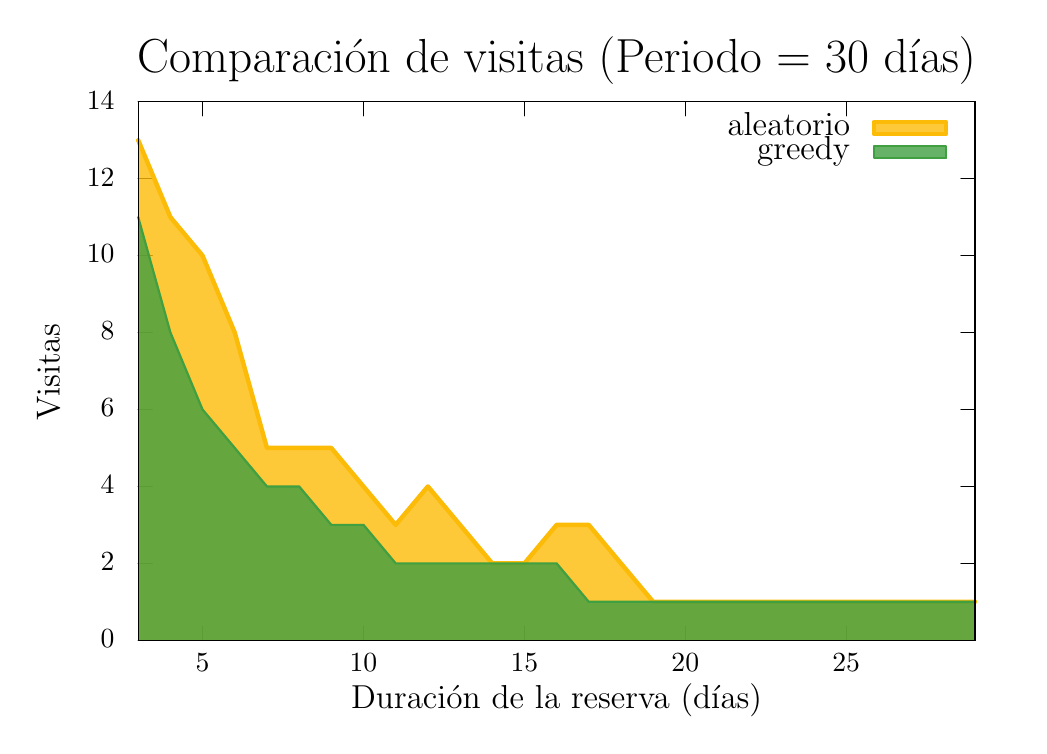
\begin{tikzpicture}[gnuplot]
%% generated with GNUPLOT 4.6p4 (Lua 5.1; terminal rev. 99, script rev. 100)
%% sáb 30 abr 2016 19:56:26 CEST
\path (0.000,0.000) rectangle (12.500,8.750);
\gpcolor{color=gp lt color border}
\gpsetlinetype{gp lt border}
\gpsetlinewidth{1.00}
\draw[gp path] (1.320,0.985)--(1.500,0.985);
\draw[gp path] (11.947,0.985)--(11.767,0.985);
\node[gp node right] at (1.136,0.985) { 0};
\draw[gp path] (1.320,1.962)--(1.500,1.962);
\draw[gp path] (11.947,1.962)--(11.767,1.962);
\node[gp node right] at (1.136,1.962) { 2};
\draw[gp path] (1.320,2.939)--(1.500,2.939);
\draw[gp path] (11.947,2.939)--(11.767,2.939);
\node[gp node right] at (1.136,2.939) { 4};
\draw[gp path] (1.320,3.916)--(1.500,3.916);
\draw[gp path] (11.947,3.916)--(11.767,3.916);
\node[gp node right] at (1.136,3.916) { 6};
\draw[gp path] (1.320,4.894)--(1.500,4.894);
\draw[gp path] (11.947,4.894)--(11.767,4.894);
\node[gp node right] at (1.136,4.894) { 8};
\draw[gp path] (1.320,5.871)--(1.500,5.871);
\draw[gp path] (11.947,5.871)--(11.767,5.871);
\node[gp node right] at (1.136,5.871) { 10};
\draw[gp path] (1.320,6.848)--(1.500,6.848);
\draw[gp path] (11.947,6.848)--(11.767,6.848);
\node[gp node right] at (1.136,6.848) { 12};
\draw[gp path] (1.320,7.825)--(1.500,7.825);
\draw[gp path] (11.947,7.825)--(11.767,7.825);
\node[gp node right] at (1.136,7.825) { 14};
\draw[gp path] (2.137,0.985)--(2.137,1.165);
\draw[gp path] (2.137,7.825)--(2.137,7.645);
\node[gp node center] at (2.137,0.677) { 5};
\draw[gp path] (4.181,0.985)--(4.181,1.165);
\draw[gp path] (4.181,7.825)--(4.181,7.645);
\node[gp node center] at (4.181,0.677) { 10};
\draw[gp path] (6.225,0.985)--(6.225,1.165);
\draw[gp path] (6.225,7.825)--(6.225,7.645);
\node[gp node center] at (6.225,0.677) { 15};
\draw[gp path] (8.268,0.985)--(8.268,1.165);
\draw[gp path] (8.268,7.825)--(8.268,7.645);
\node[gp node center] at (8.268,0.677) { 20};
\draw[gp path] (10.312,0.985)--(10.312,1.165);
\draw[gp path] (10.312,7.825)--(10.312,7.645);
\node[gp node center] at (10.312,0.677) { 25};
\draw[gp path] (1.320,7.825)--(1.320,0.985)--(11.947,0.985)--(11.947,7.825)--cycle;
\node[gp node center,rotate=-270,font={\fontsize{12pt}{14.4pt}\selectfont}] at (0.246,4.405) {Visitas};
\node[gp node center,font={\fontsize{12pt}{14.4pt}\selectfont}] at (6.633,0.215) {Duración de la reserva (días)};
\node[gp node center,font={\fontsize{16pt}{19.2pt}\selectfont}] at (6.633,8.287) {Comparación de visitas (Periodo = 30 días)};
\node[gp node right,font={\fontsize{12pt}{14.4pt}\selectfont}] at (10.479,7.491) {aleatorio};
\gpfill{rgb color={0.988,0.733,0.024},opacity=0.80} (10.663,7.414)--(11.579,7.414)--(11.579,7.568)--(10.663,7.568)--cycle;
\gpcolor{rgb color={0.988,0.733,0.024}}
\gpsetlinetype{gp lt plot 0}
\gpsetlinewidth{4.00}
\draw[gp path] (10.663,7.414)--(11.579,7.414)--(11.579,7.568)--(10.663,7.568)--cycle;
%
  \gpfill{rgb color={0.988,0.733,0.024},opacity=0.80} (1.320,7.336)--(1.320,7.336)--(1.729,6.359)--(2.137,5.871)%
    --(2.546,4.894)--(2.955,3.428)--(3.364,3.428)--(3.772,3.428)--(4.181,2.939)%
    --(4.590,2.451)--(4.999,2.939)--(5.407,2.451)--(5.816,1.962)--(6.225,1.962)%
    --(6.634,2.451)--(7.042,2.451)--(7.451,1.962)--(7.860,1.474)--(8.268,1.474)%
    --(8.677,1.474)--(9.086,1.474)--(9.495,1.474)--(9.903,1.474)--(10.312,1.474)%
    --(10.721,1.474)--(11.130,1.474)--(11.538,1.474)--(11.947,1.474)--(11.947,0.985)--(1.320,0.985)--cycle;
\draw[gp path] (1.320,7.336)--(1.729,6.359)--(2.137,5.871)--(2.546,4.894)--(2.955,3.428)%
  --(3.364,3.428)--(3.772,3.428)--(4.181,2.939)--(4.590,2.451)--(4.999,2.939)--(5.407,2.451)%
  --(5.816,1.962)--(6.225,1.962)--(6.634,2.451)--(7.042,2.451)--(7.451,1.962)--(7.860,1.474)%
  --(8.268,1.474)--(8.677,1.474)--(9.086,1.474)--(9.495,1.474)--(9.903,1.474)--(10.312,1.474)%
  --(10.721,1.474)--(11.130,1.474)--(11.538,1.474)--(11.947,1.474);
\gpcolor{color=gp lt color border}
\node[gp node right,font={\fontsize{12pt}{14.4pt}\selectfont}] at (10.479,7.183) {greedy};
\gpfill{rgb color={0.251,0.624,0.251},opacity=0.80} (10.663,7.106)--(11.579,7.106)--(11.579,7.260)--(10.663,7.260)--cycle;
\gpcolor{rgb color={0.251,0.624,0.251}}
\gpsetlinewidth{2.00}
\draw[gp path] (10.663,7.106)--(11.579,7.106)--(11.579,7.260)--(10.663,7.260)--cycle;
%
  \gpfill{rgb color={0.251,0.624,0.251},opacity=0.80} (1.320,6.359)--(1.320,6.359)--(1.729,4.894)--(2.137,3.916)%
    --(2.546,3.428)--(2.955,2.939)--(3.364,2.939)--(3.772,2.451)--(4.181,2.451)%
    --(4.590,1.962)--(4.999,1.962)--(5.407,1.962)--(5.816,1.962)--(6.225,1.962)%
    --(6.634,1.962)--(7.042,1.474)--(7.451,1.474)--(7.860,1.474)--(8.268,1.474)%
    --(8.677,1.474)--(9.086,1.474)--(9.495,1.474)--(9.903,1.474)--(10.312,1.474)%
    --(10.721,1.474)--(11.130,1.474)--(11.538,1.474)--(11.947,1.474)--(11.947,0.985)--(1.320,0.985)--cycle;
\draw[gp path] (1.320,6.359)--(1.729,4.894)--(2.137,3.916)--(2.546,3.428)--(2.955,2.939)%
  --(3.364,2.939)--(3.772,2.451)--(4.181,2.451)--(4.590,1.962)--(4.999,1.962)--(5.407,1.962)%
  --(5.816,1.962)--(6.225,1.962)--(6.634,1.962)--(7.042,1.474)--(7.451,1.474)--(7.860,1.474)%
  --(8.268,1.474)--(8.677,1.474)--(9.086,1.474)--(9.495,1.474)--(9.903,1.474)--(10.312,1.474)%
  --(10.721,1.474)--(11.130,1.474)--(11.538,1.474)--(11.947,1.474);
\gpcolor{color=gp lt color border}
\gpsetlinetype{gp lt border}
\gpsetlinewidth{1.00}
\draw[gp path] (1.320,7.825)--(1.320,0.985)--(11.947,0.985)--(11.947,7.825)--cycle;
%% coordinates of the plot area
\gpdefrectangularnode{gp plot 1}{\pgfpoint{1.320cm}{0.985cm}}{\pgfpoint{11.947cm}{7.825cm}}
\end{tikzpicture}
%% gnuplot variables
}
\end{center}

Como ya hemos probado el algoritmo greedy obtiene la mejor solución, por lo que siempre se encuentra por debajo del otro algoritmo. Además genera una gráfica descendiente, mientras que el aleatorio presenta máximos y mínimos locales.\\

Ahora fijamos la duración de la reserva en 5 días y variamos el tamaño del periodo. De esta manera obtenemos una gráfica creciente.\\

\begin{center}
\resizebox{5.3in}{!}{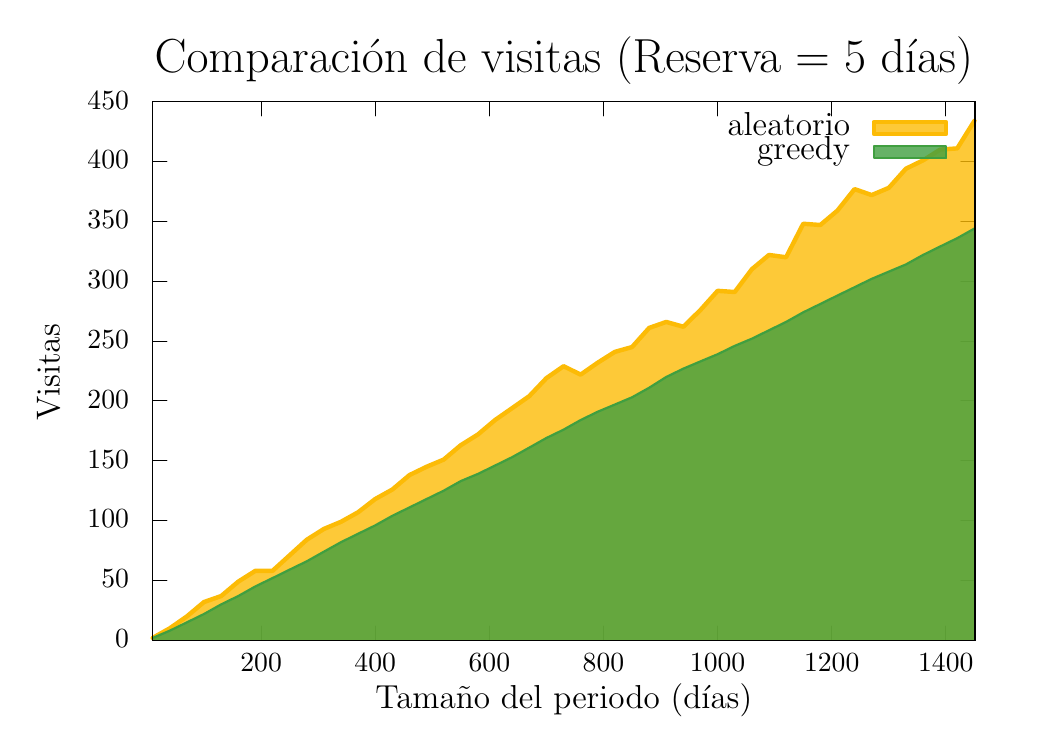
\begin{tikzpicture}[gnuplot]
%% generated with GNUPLOT 4.6p4 (Lua 5.1; terminal rev. 99, script rev. 100)
%% sáb 30 abr 2016 19:56:26 CEST
\path (0.000,0.000) rectangle (12.500,8.750);
\gpcolor{color=gp lt color border}
\gpsetlinetype{gp lt border}
\gpsetlinewidth{1.00}
\draw[gp path] (1.504,0.985)--(1.684,0.985);
\draw[gp path] (11.947,0.985)--(11.767,0.985);
\node[gp node right] at (1.320,0.985) { 0};
\draw[gp path] (1.504,1.745)--(1.684,1.745);
\draw[gp path] (11.947,1.745)--(11.767,1.745);
\node[gp node right] at (1.320,1.745) { 50};
\draw[gp path] (1.504,2.505)--(1.684,2.505);
\draw[gp path] (11.947,2.505)--(11.767,2.505);
\node[gp node right] at (1.320,2.505) { 100};
\draw[gp path] (1.504,3.265)--(1.684,3.265);
\draw[gp path] (11.947,3.265)--(11.767,3.265);
\node[gp node right] at (1.320,3.265) { 150};
\draw[gp path] (1.504,4.025)--(1.684,4.025);
\draw[gp path] (11.947,4.025)--(11.767,4.025);
\node[gp node right] at (1.320,4.025) { 200};
\draw[gp path] (1.504,4.785)--(1.684,4.785);
\draw[gp path] (11.947,4.785)--(11.767,4.785);
\node[gp node right] at (1.320,4.785) { 250};
\draw[gp path] (1.504,5.545)--(1.684,5.545);
\draw[gp path] (11.947,5.545)--(11.767,5.545);
\node[gp node right] at (1.320,5.545) { 300};
\draw[gp path] (1.504,6.305)--(1.684,6.305);
\draw[gp path] (11.947,6.305)--(11.767,6.305);
\node[gp node right] at (1.320,6.305) { 350};
\draw[gp path] (1.504,7.065)--(1.684,7.065);
\draw[gp path] (11.947,7.065)--(11.767,7.065);
\node[gp node right] at (1.320,7.065) { 400};
\draw[gp path] (1.504,7.825)--(1.684,7.825);
\draw[gp path] (11.947,7.825)--(11.767,7.825);
\node[gp node right] at (1.320,7.825) { 450};
\draw[gp path] (2.881,0.985)--(2.881,1.165);
\draw[gp path] (2.881,7.825)--(2.881,7.645);
\node[gp node center] at (2.881,0.677) { 200};
\draw[gp path] (4.330,0.985)--(4.330,1.165);
\draw[gp path] (4.330,7.825)--(4.330,7.645);
\node[gp node center] at (4.330,0.677) { 400};
\draw[gp path] (5.780,0.985)--(5.780,1.165);
\draw[gp path] (5.780,7.825)--(5.780,7.645);
\node[gp node center] at (5.780,0.677) { 600};
\draw[gp path] (7.229,0.985)--(7.229,1.165);
\draw[gp path] (7.229,7.825)--(7.229,7.645);
\node[gp node center] at (7.229,0.677) { 800};
\draw[gp path] (8.679,0.985)--(8.679,1.165);
\draw[gp path] (8.679,7.825)--(8.679,7.645);
\node[gp node center] at (8.679,0.677) { 1000};
\draw[gp path] (10.128,0.985)--(10.128,1.165);
\draw[gp path] (10.128,7.825)--(10.128,7.645);
\node[gp node center] at (10.128,0.677) { 1200};
\draw[gp path] (11.577,0.985)--(11.577,1.165);
\draw[gp path] (11.577,7.825)--(11.577,7.645);
\node[gp node center] at (11.577,0.677) { 1400};
\draw[gp path] (1.504,7.825)--(1.504,0.985)--(11.947,0.985)--(11.947,7.825)--cycle;
\node[gp node center,rotate=-270,font={\fontsize{12pt}{14.4pt}\selectfont}] at (0.246,4.405) {Visitas};
\node[gp node center,font={\fontsize{12pt}{14.4pt}\selectfont}] at (6.725,0.215) {Tamaño del periodo (días)};
\node[gp node center,font={\fontsize{16pt}{19.2pt}\selectfont}] at (6.725,8.287) {Comparación de visitas (Reserva = 5 días)};
\node[gp node right,font={\fontsize{12pt}{14.4pt}\selectfont}] at (10.479,7.491) {aleatorio};
\gpfill{rgb color={0.988,0.733,0.024},opacity=0.80} (10.663,7.414)--(11.579,7.414)--(11.579,7.568)--(10.663,7.568)--cycle;
\gpcolor{rgb color={0.988,0.733,0.024}}
\gpsetlinetype{gp lt plot 0}
\gpsetlinewidth{4.00}
\draw[gp path] (10.663,7.414)--(11.579,7.414)--(11.579,7.568)--(10.663,7.568)--cycle;
\gpfill{rgb color={0.988,0.733,0.024},opacity=0.80} (1.504,1.015)--(1.504,1.015)--(1.721,1.137)--(1.939,1.289)%
    --(2.156,1.471)--(2.374,1.547)--(2.591,1.730)--(2.808,1.867)--(3.026,1.867)%
    --(3.243,2.064)--(3.461,2.262)--(3.678,2.399)--(3.896,2.490)--(4.113,2.611)%
    --(4.330,2.779)--(4.548,2.900)--(4.765,3.083)--(4.983,3.189)--(5.200,3.280)%
    --(5.417,3.463)--(5.635,3.599)--(5.852,3.782)--(6.070,3.934)--(6.287,4.086)%
    --(6.504,4.314)--(6.722,4.466)--(6.939,4.359)--(7.157,4.511)--(7.374,4.648)%
    --(7.592,4.709)--(7.809,4.952)--(8.026,5.028)--(8.244,4.967)--(8.461,5.180)%
    --(8.679,5.423)--(8.896,5.408)--(9.113,5.697)--(9.331,5.879)--(9.548,5.849)%
    --(9.766,6.275)--(9.983,6.259)--(10.200,6.442)--(10.418,6.715)--(10.635,6.639)%
    --(10.853,6.731)--(11.070,6.974)--(11.288,7.080)--(11.505,7.217)--(11.722,7.232)%
    --(11.940,7.582)--(11.940,0.985)--(1.504,0.985)--cycle;
\draw[gp path] (1.504,1.015)--(1.721,1.137)--(1.939,1.289)--(2.156,1.471)--(2.374,1.547)%
  --(2.591,1.730)--(2.808,1.867)--(3.026,1.867)--(3.243,2.064)--(3.461,2.262)--(3.678,2.399)%
  --(3.896,2.490)--(4.113,2.611)--(4.330,2.779)--(4.548,2.900)--(4.765,3.083)--(4.983,3.189)%
  --(5.200,3.280)--(5.417,3.463)--(5.635,3.599)--(5.852,3.782)--(6.070,3.934)--(6.287,4.086)%
  --(6.504,4.314)--(6.722,4.466)--(6.939,4.359)--(7.157,4.511)--(7.374,4.648)--(7.592,4.709)%
  --(7.809,4.952)--(8.026,5.028)--(8.244,4.967)--(8.461,5.180)--(8.679,5.423)--(8.896,5.408)%
  --(9.113,5.697)--(9.331,5.879)--(9.548,5.849)--(9.766,6.275)--(9.983,6.259)--(10.200,6.442)%
  --(10.418,6.715)--(10.635,6.639)--(10.853,6.731)--(11.070,6.974)--(11.288,7.080)--(11.505,7.217)%
  --(11.722,7.232)--(11.940,7.582);
\gpcolor{color=gp lt color border}
\node[gp node right,font={\fontsize{12pt}{14.4pt}\selectfont}] at (10.479,7.183) {greedy};
\gpfill{rgb color={0.251,0.624,0.251},opacity=0.80} (10.663,7.106)--(11.579,7.106)--(11.579,7.260)--(10.663,7.260)--cycle;
\gpcolor{rgb color={0.251,0.624,0.251}}
\gpsetlinewidth{2.00}
\draw[gp path] (10.663,7.106)--(11.579,7.106)--(11.579,7.260)--(10.663,7.260)--cycle;
\gpfill{rgb color={0.251,0.624,0.251},opacity=0.80} (1.504,1.015)--(1.504,1.015)--(1.721,1.107)--(1.939,1.213)%
    --(2.156,1.319)--(2.374,1.441)--(2.591,1.547)--(2.808,1.669)--(3.026,1.775)%
    --(3.243,1.882)--(3.461,1.988)--(3.678,2.110)--(3.896,2.231)--(4.113,2.338)%
    --(4.330,2.444)--(4.548,2.566)--(4.765,2.672)--(4.983,2.779)--(5.200,2.885)%
    --(5.417,3.007)--(5.635,3.098)--(5.852,3.204)--(6.070,3.311)--(6.287,3.432)%
    --(6.504,3.554)--(6.722,3.660)--(6.939,3.782)--(7.157,3.888)--(7.374,3.979)%
    --(7.592,4.071)--(7.809,4.192)--(8.026,4.329)--(8.244,4.435)--(8.461,4.527)%
    --(8.679,4.618)--(8.896,4.724)--(9.113,4.815)--(9.331,4.922)--(9.548,5.028)%
    --(9.766,5.150)--(9.983,5.256)--(10.200,5.363)--(10.418,5.469)--(10.635,5.575)%
    --(10.853,5.667)--(11.070,5.758)--(11.288,5.879)--(11.505,5.986)--(11.722,6.092)%
    --(11.940,6.214)--(11.940,0.985)--(1.504,0.985)--cycle;
\draw[gp path] (1.504,1.015)--(1.721,1.107)--(1.939,1.213)--(2.156,1.319)--(2.374,1.441)%
  --(2.591,1.547)--(2.808,1.669)--(3.026,1.775)--(3.243,1.882)--(3.461,1.988)--(3.678,2.110)%
  --(3.896,2.231)--(4.113,2.338)--(4.330,2.444)--(4.548,2.566)--(4.765,2.672)--(4.983,2.779)%
  --(5.200,2.885)--(5.417,3.007)--(5.635,3.098)--(5.852,3.204)--(6.070,3.311)--(6.287,3.432)%
  --(6.504,3.554)--(6.722,3.660)--(6.939,3.782)--(7.157,3.888)--(7.374,3.979)--(7.592,4.071)%
  --(7.809,4.192)--(8.026,4.329)--(8.244,4.435)--(8.461,4.527)--(8.679,4.618)--(8.896,4.724)%
  --(9.113,4.815)--(9.331,4.922)--(9.548,5.028)--(9.766,5.150)--(9.983,5.256)--(10.200,5.363)%
  --(10.418,5.469)--(10.635,5.575)--(10.853,5.667)--(11.070,5.758)--(11.288,5.879)--(11.505,5.986)%
  --(11.722,6.092)--(11.940,6.214);
\gpcolor{color=gp lt color border}
\gpsetlinetype{gp lt border}
\gpsetlinewidth{1.00}
\draw[gp path] (1.504,7.825)--(1.504,0.985)--(11.947,0.985)--(11.947,7.825)--cycle;
%% coordinates of the plot area
\gpdefrectangularnode{gp plot 1}{\pgfpoint{1.504cm}{0.985cm}}{\pgfpoint{11.947cm}{7.825cm}}
\end{tikzpicture}
%% gnuplot variables
}
\end{center}

Las conclusiones son parecidas a las de la gráfica anterior. Cabe mencionar que aunque parece que las visitas aumentan de forma lineal en el algoritmo greedy, no se puede asegurar, ya que la distribución de días en los que abre la tienda es aleatoria.\\

También es interesante observar que ocurre de forma media. Para ello calculamos el número medio de visitas con una reserva aleatoria y en un periodo determinado.\\

\begin{center}
\resizebox{5.3in}{!}{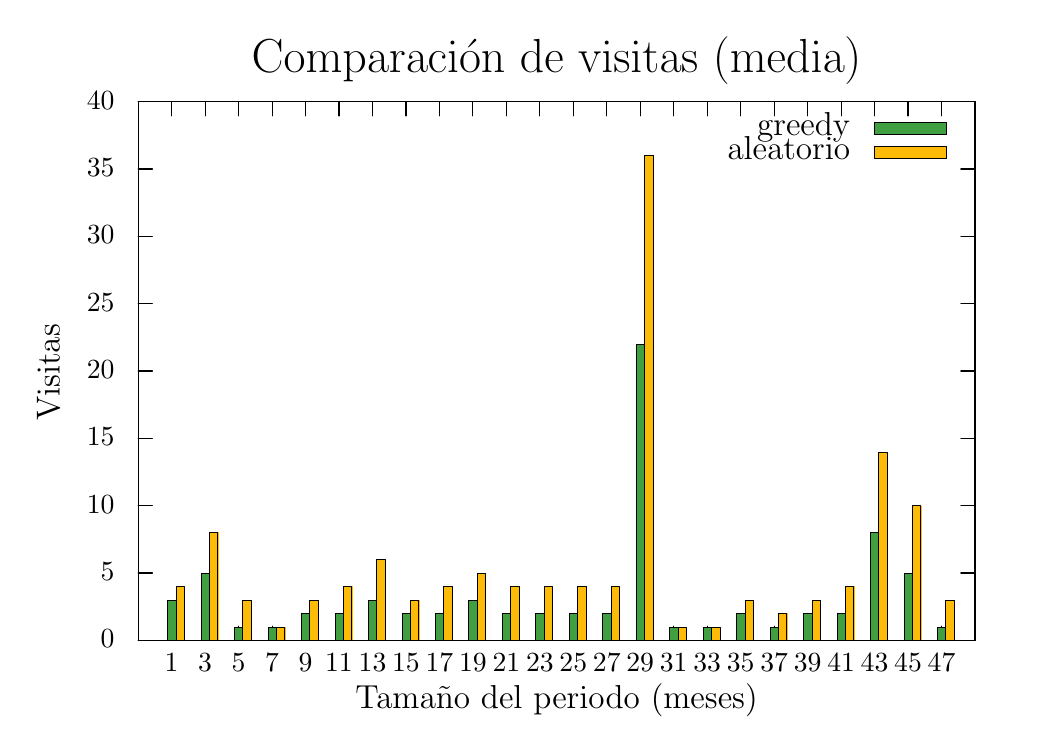
\begin{tikzpicture}[gnuplot]
%% generated with GNUPLOT 4.6p4 (Lua 5.1; terminal rev. 99, script rev. 100)
%% sáb 30 abr 2016 19:56:30 CEST
\path (0.000,0.000) rectangle (12.500,8.750);
\gpcolor{color=gp lt color border}
\gpsetlinetype{gp lt border}
\gpsetlinewidth{1.00}
\draw[gp path] (1.320,0.985)--(1.500,0.985);
\draw[gp path] (11.947,0.985)--(11.767,0.985);
\node[gp node right,font={\fontsize{10pt}{12pt}\selectfont}] at (1.136,0.985) { 0};
\draw[gp path] (1.320,1.840)--(1.500,1.840);
\draw[gp path] (11.947,1.840)--(11.767,1.840);
\node[gp node right,font={\fontsize{10pt}{12pt}\selectfont}] at (1.136,1.840) { 5};
\draw[gp path] (1.320,2.695)--(1.500,2.695);
\draw[gp path] (11.947,2.695)--(11.767,2.695);
\node[gp node right,font={\fontsize{10pt}{12pt}\selectfont}] at (1.136,2.695) { 10};
\draw[gp path] (1.320,3.550)--(1.500,3.550);
\draw[gp path] (11.947,3.550)--(11.767,3.550);
\node[gp node right,font={\fontsize{10pt}{12pt}\selectfont}] at (1.136,3.550) { 15};
\draw[gp path] (1.320,4.405)--(1.500,4.405);
\draw[gp path] (11.947,4.405)--(11.767,4.405);
\node[gp node right,font={\fontsize{10pt}{12pt}\selectfont}] at (1.136,4.405) { 20};
\draw[gp path] (1.320,5.260)--(1.500,5.260);
\draw[gp path] (11.947,5.260)--(11.767,5.260);
\node[gp node right,font={\fontsize{10pt}{12pt}\selectfont}] at (1.136,5.260) { 25};
\draw[gp path] (1.320,6.115)--(1.500,6.115);
\draw[gp path] (11.947,6.115)--(11.767,6.115);
\node[gp node right,font={\fontsize{10pt}{12pt}\selectfont}] at (1.136,6.115) { 30};
\draw[gp path] (1.320,6.970)--(1.500,6.970);
\draw[gp path] (11.947,6.970)--(11.767,6.970);
\node[gp node right,font={\fontsize{10pt}{12pt}\selectfont}] at (1.136,6.970) { 35};
\draw[gp path] (1.320,7.825)--(1.500,7.825);
\draw[gp path] (11.947,7.825)--(11.767,7.825);
\node[gp node right,font={\fontsize{10pt}{12pt}\selectfont}] at (1.136,7.825) { 40};
\draw[gp path] (1.745,0.985)--(1.745,1.165);
\draw[gp path] (1.745,7.825)--(1.745,7.645);
\node[gp node center,font={\fontsize{10pt}{12pt}\selectfont}] at (1.745,0.677) {1};
\draw[gp path] (2.170,0.985)--(2.170,1.165);
\draw[gp path] (2.170,7.825)--(2.170,7.645);
\node[gp node center,font={\fontsize{10pt}{12pt}\selectfont}] at (2.170,0.677) {3};
\draw[gp path] (2.595,0.985)--(2.595,1.165);
\draw[gp path] (2.595,7.825)--(2.595,7.645);
\node[gp node center,font={\fontsize{10pt}{12pt}\selectfont}] at (2.595,0.677) {5};
\draw[gp path] (3.020,0.985)--(3.020,1.165);
\draw[gp path] (3.020,7.825)--(3.020,7.645);
\node[gp node center,font={\fontsize{10pt}{12pt}\selectfont}] at (3.020,0.677) {7};
\draw[gp path] (3.445,0.985)--(3.445,1.165);
\draw[gp path] (3.445,7.825)--(3.445,7.645);
\node[gp node center,font={\fontsize{10pt}{12pt}\selectfont}] at (3.445,0.677) {9};
\draw[gp path] (3.870,0.985)--(3.870,1.165);
\draw[gp path] (3.870,7.825)--(3.870,7.645);
\node[gp node center,font={\fontsize{10pt}{12pt}\selectfont}] at (3.870,0.677) {11};
\draw[gp path] (4.296,0.985)--(4.296,1.165);
\draw[gp path] (4.296,7.825)--(4.296,7.645);
\node[gp node center,font={\fontsize{10pt}{12pt}\selectfont}] at (4.296,0.677) {13};
\draw[gp path] (4.721,0.985)--(4.721,1.165);
\draw[gp path] (4.721,7.825)--(4.721,7.645);
\node[gp node center,font={\fontsize{10pt}{12pt}\selectfont}] at (4.721,0.677) {15};
\draw[gp path] (5.146,0.985)--(5.146,1.165);
\draw[gp path] (5.146,7.825)--(5.146,7.645);
\node[gp node center,font={\fontsize{10pt}{12pt}\selectfont}] at (5.146,0.677) {17};
\draw[gp path] (5.571,0.985)--(5.571,1.165);
\draw[gp path] (5.571,7.825)--(5.571,7.645);
\node[gp node center,font={\fontsize{10pt}{12pt}\selectfont}] at (5.571,0.677) {19};
\draw[gp path] (5.996,0.985)--(5.996,1.165);
\draw[gp path] (5.996,7.825)--(5.996,7.645);
\node[gp node center,font={\fontsize{10pt}{12pt}\selectfont}] at (5.996,0.677) {21};
\draw[gp path] (6.421,0.985)--(6.421,1.165);
\draw[gp path] (6.421,7.825)--(6.421,7.645);
\node[gp node center,font={\fontsize{10pt}{12pt}\selectfont}] at (6.421,0.677) {23};
\draw[gp path] (6.846,0.985)--(6.846,1.165);
\draw[gp path] (6.846,7.825)--(6.846,7.645);
\node[gp node center,font={\fontsize{10pt}{12pt}\selectfont}] at (6.846,0.677) {25};
\draw[gp path] (7.271,0.985)--(7.271,1.165);
\draw[gp path] (7.271,7.825)--(7.271,7.645);
\node[gp node center,font={\fontsize{10pt}{12pt}\selectfont}] at (7.271,0.677) {27};
\draw[gp path] (7.696,0.985)--(7.696,1.165);
\draw[gp path] (7.696,7.825)--(7.696,7.645);
\node[gp node center,font={\fontsize{10pt}{12pt}\selectfont}] at (7.696,0.677) {29};
\draw[gp path] (8.121,0.985)--(8.121,1.165);
\draw[gp path] (8.121,7.825)--(8.121,7.645);
\node[gp node center,font={\fontsize{10pt}{12pt}\selectfont}] at (8.121,0.677) {31};
\draw[gp path] (8.546,0.985)--(8.546,1.165);
\draw[gp path] (8.546,7.825)--(8.546,7.645);
\node[gp node center,font={\fontsize{10pt}{12pt}\selectfont}] at (8.546,0.677) {33};
\draw[gp path] (8.971,0.985)--(8.971,1.165);
\draw[gp path] (8.971,7.825)--(8.971,7.645);
\node[gp node center,font={\fontsize{10pt}{12pt}\selectfont}] at (8.971,0.677) {35};
\draw[gp path] (9.397,0.985)--(9.397,1.165);
\draw[gp path] (9.397,7.825)--(9.397,7.645);
\node[gp node center,font={\fontsize{10pt}{12pt}\selectfont}] at (9.397,0.677) {37};
\draw[gp path] (9.822,0.985)--(9.822,1.165);
\draw[gp path] (9.822,7.825)--(9.822,7.645);
\node[gp node center,font={\fontsize{10pt}{12pt}\selectfont}] at (9.822,0.677) {39};
\draw[gp path] (10.247,0.985)--(10.247,1.165);
\draw[gp path] (10.247,7.825)--(10.247,7.645);
\node[gp node center,font={\fontsize{10pt}{12pt}\selectfont}] at (10.247,0.677) {41};
\draw[gp path] (10.672,0.985)--(10.672,1.165);
\draw[gp path] (10.672,7.825)--(10.672,7.645);
\node[gp node center,font={\fontsize{10pt}{12pt}\selectfont}] at (10.672,0.677) {43};
\draw[gp path] (11.097,0.985)--(11.097,1.165);
\draw[gp path] (11.097,7.825)--(11.097,7.645);
\node[gp node center,font={\fontsize{10pt}{12pt}\selectfont}] at (11.097,0.677) {45};
\draw[gp path] (11.522,0.985)--(11.522,1.165);
\draw[gp path] (11.522,7.825)--(11.522,7.645);
\node[gp node center,font={\fontsize{10pt}{12pt}\selectfont}] at (11.522,0.677) {47};
\draw[gp path] (1.320,7.825)--(1.320,0.985)--(11.947,0.985)--(11.947,7.825)--cycle;
\node[gp node center,rotate=-270,font={\fontsize{12pt}{14.4pt}\selectfont}] at (0.246,4.405) {Visitas};
\node[gp node center,font={\fontsize{12pt}{14.4pt}\selectfont}] at (6.633,0.215) {Tamaño del periodo (meses)};
\node[gp node center,font={\fontsize{16pt}{19.2pt}\selectfont}] at (6.633,8.287) {Comparación de visitas (media)};
\node[gp node right,font={\fontsize{12pt}{14.4pt}\selectfont}] at (10.479,7.491) {greedy};
\gpfill{rgb color={0.251,0.624,0.251}} (10.663,7.414)--(11.579,7.414)--(11.579,7.568)--(10.663,7.568)--cycle;
\gpsetlinetype{gp lt plot 0}
\gpsetlinewidth{0.50}
\draw[gp path] (10.663,7.414)--(11.579,7.414)--(11.579,7.568)--(10.663,7.568)--cycle;
\gpfill{rgb color={0.251,0.624,0.251}} (1.692,0.985)--(1.799,0.985)--(1.799,1.499)--(1.692,1.499)--cycle;
\draw[gp path] (1.692,0.985)--(1.692,1.498)--(1.798,1.498)--(1.798,0.985)--cycle;
\gpfill{rgb color={0.251,0.624,0.251}} (2.117,0.985)--(2.224,0.985)--(2.224,1.841)--(2.117,1.841)--cycle;
\draw[gp path] (2.117,0.985)--(2.117,1.840)--(2.223,1.840)--(2.223,0.985)--cycle;
\gpfill{rgb color={0.251,0.624,0.251}} (2.542,0.985)--(2.649,0.985)--(2.649,1.157)--(2.542,1.157)--cycle;
\draw[gp path] (2.542,0.985)--(2.542,1.156)--(2.648,1.156)--(2.648,0.985)--cycle;
\gpfill{rgb color={0.251,0.624,0.251}} (2.967,0.985)--(3.074,0.985)--(3.074,1.157)--(2.967,1.157)--cycle;
\draw[gp path] (2.967,0.985)--(2.967,1.156)--(3.073,1.156)--(3.073,0.985)--cycle;
\gpfill{rgb color={0.251,0.624,0.251}} (3.392,0.985)--(3.500,0.985)--(3.500,1.328)--(3.392,1.328)--cycle;
\draw[gp path] (3.392,0.985)--(3.392,1.327)--(3.499,1.327)--(3.499,0.985)--cycle;
\gpfill{rgb color={0.251,0.624,0.251}} (3.817,0.985)--(3.925,0.985)--(3.925,1.328)--(3.817,1.328)--cycle;
\draw[gp path] (3.817,0.985)--(3.817,1.327)--(3.924,1.327)--(3.924,0.985)--cycle;
\gpfill{rgb color={0.251,0.624,0.251}} (4.242,0.985)--(4.350,0.985)--(4.350,1.499)--(4.242,1.499)--cycle;
\draw[gp path] (4.242,0.985)--(4.242,1.498)--(4.349,1.498)--(4.349,0.985)--cycle;
\gpfill{rgb color={0.251,0.624,0.251}} (4.668,0.985)--(4.775,0.985)--(4.775,1.328)--(4.668,1.328)--cycle;
\draw[gp path] (4.668,0.985)--(4.668,1.327)--(4.774,1.327)--(4.774,0.985)--cycle;
\gpfill{rgb color={0.251,0.624,0.251}} (5.093,0.985)--(5.200,0.985)--(5.200,1.328)--(5.093,1.328)--cycle;
\draw[gp path] (5.093,0.985)--(5.093,1.327)--(5.199,1.327)--(5.199,0.985)--cycle;
\gpfill{rgb color={0.251,0.624,0.251}} (5.518,0.985)--(5.625,0.985)--(5.625,1.499)--(5.518,1.499)--cycle;
\draw[gp path] (5.518,0.985)--(5.518,1.498)--(5.624,1.498)--(5.624,0.985)--cycle;
\gpfill{rgb color={0.251,0.624,0.251}} (5.943,0.985)--(6.050,0.985)--(6.050,1.328)--(5.943,1.328)--cycle;
\draw[gp path] (5.943,0.985)--(5.943,1.327)--(6.049,1.327)--(6.049,0.985)--cycle;
\gpfill{rgb color={0.251,0.624,0.251}} (6.368,0.985)--(6.475,0.985)--(6.475,1.328)--(6.368,1.328)--cycle;
\draw[gp path] (6.368,0.985)--(6.368,1.327)--(6.474,1.327)--(6.474,0.985)--cycle;
\gpfill{rgb color={0.251,0.624,0.251}} (6.793,0.985)--(6.900,0.985)--(6.900,1.328)--(6.793,1.328)--cycle;
\draw[gp path] (6.793,0.985)--(6.793,1.327)--(6.899,1.327)--(6.899,0.985)--cycle;
\gpfill{rgb color={0.251,0.624,0.251}} (7.218,0.985)--(7.325,0.985)--(7.325,1.328)--(7.218,1.328)--cycle;
\draw[gp path] (7.218,0.985)--(7.218,1.327)--(7.324,1.327)--(7.324,0.985)--cycle;
\gpfill{rgb color={0.251,0.624,0.251}} (7.643,0.985)--(7.750,0.985)--(7.750,4.748)--(7.643,4.748)--cycle;
\draw[gp path] (7.643,0.985)--(7.643,4.747)--(7.749,4.747)--(7.749,0.985)--cycle;
\gpfill{rgb color={0.251,0.624,0.251}} (8.068,0.985)--(8.175,0.985)--(8.175,1.157)--(8.068,1.157)--cycle;
\draw[gp path] (8.068,0.985)--(8.068,1.156)--(8.174,1.156)--(8.174,0.985)--cycle;
\gpfill{rgb color={0.251,0.624,0.251}} (8.493,0.985)--(8.600,0.985)--(8.600,1.157)--(8.493,1.157)--cycle;
\draw[gp path] (8.493,0.985)--(8.493,1.156)--(8.599,1.156)--(8.599,0.985)--cycle;
\gpfill{rgb color={0.251,0.624,0.251}} (8.918,0.985)--(9.026,0.985)--(9.026,1.328)--(8.918,1.328)--cycle;
\draw[gp path] (8.918,0.985)--(8.918,1.327)--(9.025,1.327)--(9.025,0.985)--cycle;
\gpfill{rgb color={0.251,0.624,0.251}} (9.343,0.985)--(9.451,0.985)--(9.451,1.157)--(9.343,1.157)--cycle;
\draw[gp path] (9.343,0.985)--(9.343,1.156)--(9.450,1.156)--(9.450,0.985)--cycle;
\gpfill{rgb color={0.251,0.624,0.251}} (9.768,0.985)--(9.876,0.985)--(9.876,1.328)--(9.768,1.328)--cycle;
\draw[gp path] (9.768,0.985)--(9.768,1.327)--(9.875,1.327)--(9.875,0.985)--cycle;
\gpfill{rgb color={0.251,0.624,0.251}} (10.194,0.985)--(10.301,0.985)--(10.301,1.328)--(10.194,1.328)--cycle;
\draw[gp path] (10.194,0.985)--(10.194,1.327)--(10.300,1.327)--(10.300,0.985)--cycle;
\gpfill{rgb color={0.251,0.624,0.251}} (10.619,0.985)--(10.726,0.985)--(10.726,2.354)--(10.619,2.354)--cycle;
\draw[gp path] (10.619,0.985)--(10.619,2.353)--(10.725,2.353)--(10.725,0.985)--cycle;
\gpfill{rgb color={0.251,0.624,0.251}} (11.044,0.985)--(11.151,0.985)--(11.151,1.841)--(11.044,1.841)--cycle;
\draw[gp path] (11.044,0.985)--(11.044,1.840)--(11.150,1.840)--(11.150,0.985)--cycle;
\gpfill{rgb color={0.251,0.624,0.251}} (11.469,0.985)--(11.576,0.985)--(11.576,1.157)--(11.469,1.157)--cycle;
\draw[gp path] (11.469,0.985)--(11.469,1.156)--(11.575,1.156)--(11.575,0.985)--cycle;
\node[gp node right,font={\fontsize{12pt}{14.4pt}\selectfont}] at (10.479,7.183) {aleatorio};
\gpfill{rgb color={0.988,0.733,0.024}} (10.663,7.106)--(11.579,7.106)--(11.579,7.260)--(10.663,7.260)--cycle;
\draw[gp path] (10.663,7.106)--(11.579,7.106)--(11.579,7.260)--(10.663,7.260)--cycle;
\gpfill{rgb color={0.988,0.733,0.024}} (1.798,0.985)--(1.905,0.985)--(1.905,1.670)--(1.798,1.670)--cycle;
\draw[gp path] (1.798,0.985)--(1.798,1.669)--(1.904,1.669)--(1.904,0.985)--cycle;
\gpfill{rgb color={0.988,0.733,0.024}} (2.223,0.985)--(2.331,0.985)--(2.331,2.354)--(2.223,2.354)--cycle;
\draw[gp path] (2.223,0.985)--(2.223,2.353)--(2.330,2.353)--(2.330,0.985)--cycle;
\gpfill{rgb color={0.988,0.733,0.024}} (2.648,0.985)--(2.756,0.985)--(2.756,1.499)--(2.648,1.499)--cycle;
\draw[gp path] (2.648,0.985)--(2.648,1.498)--(2.755,1.498)--(2.755,0.985)--cycle;
\gpfill{rgb color={0.988,0.733,0.024}} (3.073,0.985)--(3.181,0.985)--(3.181,1.157)--(3.073,1.157)--cycle;
\draw[gp path] (3.073,0.985)--(3.073,1.156)--(3.180,1.156)--(3.180,0.985)--cycle;
\gpfill{rgb color={0.988,0.733,0.024}} (3.499,0.985)--(3.606,0.985)--(3.606,1.499)--(3.499,1.499)--cycle;
\draw[gp path] (3.499,0.985)--(3.499,1.498)--(3.605,1.498)--(3.605,0.985)--cycle;
\gpfill{rgb color={0.988,0.733,0.024}} (3.924,0.985)--(4.031,0.985)--(4.031,1.670)--(3.924,1.670)--cycle;
\draw[gp path] (3.924,0.985)--(3.924,1.669)--(4.030,1.669)--(4.030,0.985)--cycle;
\gpfill{rgb color={0.988,0.733,0.024}} (4.349,0.985)--(4.456,0.985)--(4.456,2.012)--(4.349,2.012)--cycle;
\draw[gp path] (4.349,0.985)--(4.349,2.011)--(4.455,2.011)--(4.455,0.985)--cycle;
\gpfill{rgb color={0.988,0.733,0.024}} (4.774,0.985)--(4.881,0.985)--(4.881,1.499)--(4.774,1.499)--cycle;
\draw[gp path] (4.774,0.985)--(4.774,1.498)--(4.880,1.498)--(4.880,0.985)--cycle;
\gpfill{rgb color={0.988,0.733,0.024}} (5.199,0.985)--(5.306,0.985)--(5.306,1.670)--(5.199,1.670)--cycle;
\draw[gp path] (5.199,0.985)--(5.199,1.669)--(5.305,1.669)--(5.305,0.985)--cycle;
\gpfill{rgb color={0.988,0.733,0.024}} (5.624,0.985)--(5.731,0.985)--(5.731,1.841)--(5.624,1.841)--cycle;
\draw[gp path] (5.624,0.985)--(5.624,1.840)--(5.730,1.840)--(5.730,0.985)--cycle;
\gpfill{rgb color={0.988,0.733,0.024}} (6.049,0.985)--(6.156,0.985)--(6.156,1.670)--(6.049,1.670)--cycle;
\draw[gp path] (6.049,0.985)--(6.049,1.669)--(6.155,1.669)--(6.155,0.985)--cycle;
\gpfill{rgb color={0.988,0.733,0.024}} (6.474,0.985)--(6.581,0.985)--(6.581,1.670)--(6.474,1.670)--cycle;
\draw[gp path] (6.474,0.985)--(6.474,1.669)--(6.580,1.669)--(6.580,0.985)--cycle;
\gpfill{rgb color={0.988,0.733,0.024}} (6.899,0.985)--(7.006,0.985)--(7.006,1.670)--(6.899,1.670)--cycle;
\draw[gp path] (6.899,0.985)--(6.899,1.669)--(7.005,1.669)--(7.005,0.985)--cycle;
\gpfill{rgb color={0.988,0.733,0.024}} (7.324,0.985)--(7.432,0.985)--(7.432,1.670)--(7.324,1.670)--cycle;
\draw[gp path] (7.324,0.985)--(7.324,1.669)--(7.431,1.669)--(7.431,0.985)--cycle;
\gpfill{rgb color={0.988,0.733,0.024}} (7.749,0.985)--(7.857,0.985)--(7.857,7.142)--(7.749,7.142)--cycle;
\draw[gp path] (7.749,0.985)--(7.749,7.141)--(7.856,7.141)--(7.856,0.985)--cycle;
\gpfill{rgb color={0.988,0.733,0.024}} (8.174,0.985)--(8.282,0.985)--(8.282,1.157)--(8.174,1.157)--cycle;
\draw[gp path] (8.174,0.985)--(8.174,1.156)--(8.281,1.156)--(8.281,0.985)--cycle;
\gpfill{rgb color={0.988,0.733,0.024}} (8.599,0.985)--(8.707,0.985)--(8.707,1.157)--(8.599,1.157)--cycle;
\draw[gp path] (8.599,0.985)--(8.599,1.156)--(8.706,1.156)--(8.706,0.985)--cycle;
\gpfill{rgb color={0.988,0.733,0.024}} (9.025,0.985)--(9.132,0.985)--(9.132,1.499)--(9.025,1.499)--cycle;
\draw[gp path] (9.025,0.985)--(9.025,1.498)--(9.131,1.498)--(9.131,0.985)--cycle;
\gpfill{rgb color={0.988,0.733,0.024}} (9.450,0.985)--(9.557,0.985)--(9.557,1.328)--(9.450,1.328)--cycle;
\draw[gp path] (9.450,0.985)--(9.450,1.327)--(9.556,1.327)--(9.556,0.985)--cycle;
\gpfill{rgb color={0.988,0.733,0.024}} (9.875,0.985)--(9.982,0.985)--(9.982,1.499)--(9.875,1.499)--cycle;
\draw[gp path] (9.875,0.985)--(9.875,1.498)--(9.981,1.498)--(9.981,0.985)--cycle;
\gpfill{rgb color={0.988,0.733,0.024}} (10.300,0.985)--(10.407,0.985)--(10.407,1.670)--(10.300,1.670)--cycle;
\draw[gp path] (10.300,0.985)--(10.300,1.669)--(10.406,1.669)--(10.406,0.985)--cycle;
\gpfill{rgb color={0.988,0.733,0.024}} (10.725,0.985)--(10.832,0.985)--(10.832,3.380)--(10.725,3.380)--cycle;
\draw[gp path] (10.725,0.985)--(10.725,3.379)--(10.831,3.379)--(10.831,0.985)--cycle;
\gpfill{rgb color={0.988,0.733,0.024}} (11.150,0.985)--(11.257,0.985)--(11.257,2.696)--(11.150,2.696)--cycle;
\draw[gp path] (11.150,0.985)--(11.150,2.695)--(11.256,2.695)--(11.256,0.985)--cycle;
\gpfill{rgb color={0.988,0.733,0.024}} (11.575,0.985)--(11.682,0.985)--(11.682,1.499)--(11.575,1.499)--cycle;
\draw[gp path] (11.575,0.985)--(11.575,1.498)--(11.681,1.498)--(11.681,0.985)--cycle;
\gpsetlinetype{gp lt border}
\gpsetlinewidth{1.00}
\draw[gp path] (1.320,7.825)--(1.320,0.985)--(11.947,0.985)--(11.947,7.825)--cycle;
%% coordinates of the plot area
\gpdefrectangularnode{gp plot 1}{\pgfpoint{1.320cm}{0.985cm}}{\pgfpoint{11.947cm}{7.825cm}}
\end{tikzpicture}
%% gnuplot variables
}
\end{center}

Podemos observar dos conclusiones muy interesantes.\\

Primero, parece que hay una proporción entre el número de visitas medio del greedy y del aleatorio, aproximadamente $\frac{2}{3}$.\\

Segundo, el tamaño del periodo no influye en el número de visitas, ya que lo realmente importante es la proporción entre el periodo y la reserva y al ser esta última la media entre 1 y p las visitas se estabilizan (salvo excepciones de la probabilidad).
\newpage

%%%%%%%%%%%%%%%%%%%%%%%%%%%%%%%%%%%%%%%%%%%%%%%%%%%%%%%%%%%%%%%%%%%%%%%%%%%%%%%%%%

\section{Viajante de comercio}
\subsection{Enunciado}
En su formulación más sencilla, el problema del viajante de comercio (TSP, por Traveling
Salesman Problem) se define como sigue: dado un conjunto de ciudades y una matriz con
las distancias entre todas ellas, un viajante debe recorrer todas las ciudades exactamente una
vez, regresando al punto de partida, de forma tal que la distancia recorrida sea mínima. 
Mas formalmente, dado un grafo $G$, conexo y ponderado, se trata de hallar el ciclo hamiltoniano de
mínimo peso de ese grafo.

Una solución para TSP es una permutación del conjunto de ciudades que indica el orden
en que se deben recorrer. Para el cálculo de la longitud del ciclo no debemos olvidar sumar la
distancia que existe entre la última ciudad y la primera (hay que cerrar el ciclo).

Por su interés teórico y práctico, existe una variedad muy amplia de algoritmos para abordar
la solución del TSP y sus variantes (siendo un problema NP-Completo, el diseño y aplicación
de algoritmos exactos para su resolución no es factible en problemas de cierto tamaño). Nos
centraremos en una serie de algoritmos aproximados de tipo greedy y evaluaremos su rendimiento
en un conjunto de instancias del TSP. Para el diseño de estos algoritmos, utilizaremos
dos enfoques diferentes: a) estrategias basadas en alguna noción de cercanía, y b) estrategias
de inserción.

En el primer caso emplearemos la heurística del vecino más cercano, cuyo funcionamiento
es extremadamente simple: dada una ciudad inicial $v_0$, se agrega como ciudad siguiente aquella
$v_i$ (no incluída en el circuito) que se encuentre más cercana a $v_0$. El procedimiento se repite
hasta que todas las ciudades se hayan visitado.

En las estrategias de inserción, la idea es comenzar con un recorrido parcial, que incluya
algunas de las ciudades, y luego extender este recorrido insertando las ciudades restantes mediante
algún criterio de tipo greedy. Para poder implementar este tipo de estrategia, deben
definirse tres elementos:

1. Cómo se construye el recorrido parcial inicial.

2. Cuál es el nodo siguiente a insertar en el recorrido parcial.

3. Dónde se inserta el nodo seleccionado.

El recorrido inicial se puede construir a partir de las tres ciudades que formen un triángulo
lo más grande posible: por ejemplo, eligiendo la ciudad que está más al Este, la que está más al
Oeste, y la que está más al norte.

Cuando se haya seleccionado una ciudad, esta se ubicará en el punto del circuito que provoque
el menor incremento de su longitud total. Es decir, hemos que comprobar, para cada
posible posición, la longitud del circuito resultante y quedarnos con la mejor alternativa.

Por último, para decidir cuál es la ciudad que añadiremos a nuestro circuito, podemos
aplicar el siguiente criterio, denominado inserción más económica: de entre todas las ciudades
no visitadas, elegimos aquella que provoque el menor incremento en la longitud total del circuito.
En otras palabras, cada ciudad debemos insertarla en cada una de las soluciones posibles y
quedarnos con la ciudad (y posición) que nos permita obtener un circuito de menor longitud.
Seleccionaremos aquella ciudad que nos proporcione el mínimo de los mínimos calculados para
cada una de las ciudades.


\subsection{Vecino más cercano}
\subsubsection{Explicación}
Esta es una de las formas más sencillas de abordar el problema del viajante.

Primero escogeremos una ciudad de inicio. Después de ello calculamos las distancias de esa ciudad al resto y escogemos la más cercana.
En el programa usado de ejemplo la clase grafo almacena los puntos (sus coordenadas) y la matriz de adyacencia del grafo, por tanto no 
tendremos que calcular repetidas veces las distancias. 
Para el algoritmo hemos usado una clase Punto y otra clase Grafo.

\begin{figure}[htbH] 
	\centering
	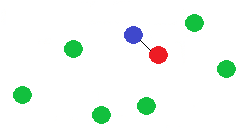
\includegraphics[width=0.5\textwidth]{./Imagenes/vecino1.png}
	\caption{Eligiendo punto de inicio en azul} 
\end{figure}

Estamos utilizando un enfoque greedy, calculando una solución óptima en cada paso local, con la experanza de llegar a una solución que se
acerque al óptimo (o lo sea, en algunos casos). Repetimos el mismo paso con cada punto:

\begin{figure}[htbH] 
	\centering
	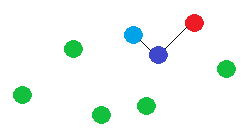
\includegraphics[width=0.5\textwidth]{./Imagenes/vecino2.png}
	\caption{Tercer vértice} 
\end{figure}

\vspace{0.5cm}
\begin{figure}[htbH] 
	\centering
	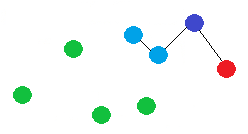
\includegraphics[width=0.5\textwidth]{./Imagenes/vecino3.png}
	\caption{Cuarto vértice} 
\end{figure}

\vspace{0.5cm}
\begin{figure}[htbH] 
	\centering
	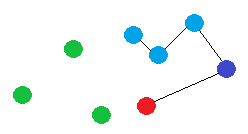
\includegraphics[width=0.5\textwidth]{./Imagenes/vecino4.png}
	\caption{Quinto vértice} 
\end{figure}

\vspace{0.5cm}
\begin{figure}[htbH] 
	\centering
	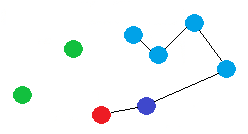
\includegraphics[width=0.5\textwidth]{./Imagenes/vecino5.png}
	\caption{Sexto vértice} 
\end{figure}

\vspace{0.5cm}
\begin{figure}[htbH] 
	\centering
	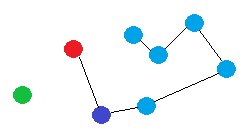
\includegraphics[width=0.5\textwidth]{./Imagenes/vecino6.png}
	\caption{Séptimo vértice} 
\end{figure}

\vspace{0.5cm}
\begin{figure}[htbH] 
	\centering
	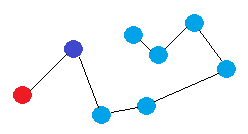
\includegraphics[width=0.5\textwidth]{./Imagenes/vecino7.png}
	\caption{Octavo y último vértice} 
\end{figure}

No debemos olvidar incluir el camino del último vértice al inicial, ya que forma parte del problema y hay que sumar también esa distancia.

\begin{figure}[htbH] 
	\centering
	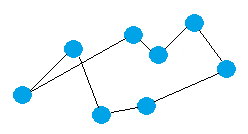
\includegraphics[width=0.5\textwidth]{./Imagenes/vecino8.png}
	\caption{Recorrido vecino más cercano} 
\end{figure}

El número de caminos (aristas) que debe recorrer coincide con el número de ciudades.
Esta solución es muy rápida de implementar y nos da una solución cercana a la óptima, pero no tiene porque ser la óptima.

\newpage


\newpage
\subsubsection{Eficiencia}
Siendo $n$ el número de ciudades por las que nuestro viajero debe pasar, denotamos cada una como $x_i=(i_a, i_b)$, $i\in\{0,1,...,n-1\}$
Definimos $\phi (x):\mathbb{N} \rightarrow \mathbb{N}$ como la función que dado un vértice o ciudad $x_i$ nos devuelve el 
índice de la ciudad más cercana, siendo su eficiencia lineal. Una vez iniciado el algoritmo nos interesará que solamente calcule
el mínimo de las distancias con las ciudades que aún no ha recorrido.
\[\phi (x_i) = \{j \in\{0,1,...,n-1\}-\{i\} : min\{dist(x_i, x_j)\} \}\]
donde 
\[ dist(x_i, x_j) = \sqrt{(i_a-j_a)^2+(i_b-j_b)^2} \]

Tenemos que pasar por las $n$ ciudades, por lo que podríamos pensar que su eficiencia es:
\[O(n) = \sum_{k=0}^{n-1} \phi (x_k)  \]

Sin embargo el algoritmo que buscamos no es tan bueno como el cuadrático, ya que tenemos una restricción. En cada paso el cálculo
del mínimo tiene que comprobar que la nueva ciudad no forme ciclo (pasaríamos dos veces por la misma ciudad).
Por tanto definimos $A$ como el conjunto de los índices de las ciudades que no han sido visitadas aún.
\[\phi '(x_i) = \{j \in A : min\{dist(x_i, x_j)\} \ y \ no \ forme \ ciclos \}\]

Comprobar si una ciudad forma ciclos es constante, por lo que tenemos que $\phi '(x_i)$ es lineal.
La eficiencia del vecino más cercano queda definida como sigue:

\[ O(n) = \sum_{k=0}^{n-1} O(\phi ' (x_k)) = n^2\]

\newpage
\subsubsection{Ejemplos}
Puntos:

	\begin{figure}[htbH]
		\centering
		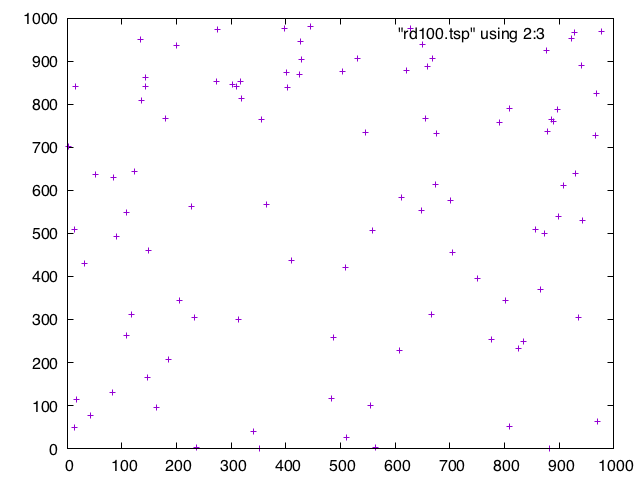
\includegraphics[width=0.65\textwidth]{../Viajante/Imagenes/rd100.png}
		\caption{Quinto vértice}
	\end{figure}
	
Recorrido óptimo:

	\begin{figure}[htbH]
		\centering
		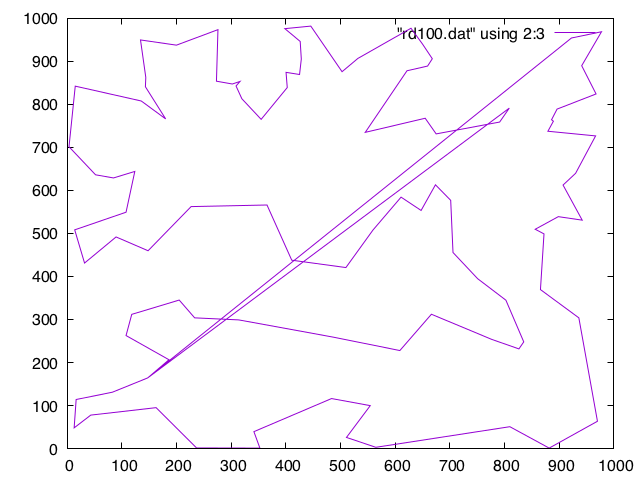
\includegraphics[width=0.65\textwidth]{../Viajante/Imagenes/rd100_opt.png}
		\caption{Quinto vértice}
	\end{figure}
\newpage

\subsection{Inserción}
\subsubsection{Explicación}
El recorrido parcial inicial lo determinan los 3 puntos que estén más al Este, Oeste y Norte respectivamente. La única restricción es que los 3 no sean los mismos, algo que nunca pasa, pues 2 de ellos pueden ser iguales (un punto puede ser a la vez el punto más al Norte y al Este), pero 3 a la vez no.

EL nodo siguiente a insertar en el recorrido parcial será un nodo arbitrario, de lo que nos encargaremos para hacer funcionar el greedy es de insertarlo entre los dos vértices que más convengan, minimizar la distancia del circuito resultante.

Pasaremos por todos los vértices que nos quedan cada vez, y sobre cada uno calculamos la posición que más nos convenga dentro del circuito, y luego escogemos el vértice que nos da mejor resultado.

\subsubsection{Eficiencia}
Tenemos que recorrer $n$ vértices, y sobre cada uno de ellos aplicaremos una función $\phi(x)$ para cada vértice.

\[ \sum_{i=1}^{n} \phi(x_i)\]

Dicha función $\phi(x)$ llama a "buscar punto" que es lineal, cada vez que buscas un punto llama $n$ veces a "buscar posicion", que a su vez llama $n$ veces a calcular longitud.

Por tanto $\phi(x)$ es cúbica, y la eficiencia que nos queda para el algoritmo de inserción es
\[ O(n) = n^4 \]

\subsection{Arista más corta}

\subsubsection{Explicación}
En este caso escogeremos una técnica greedy diferente.
Para intentar mejorar las estrategias del vecino más cercano y la inserción de vértices nos centraremos en una estrategia que consiste en ir seleccionando las aristas de menor longitud.

Primero crearemos una clase Arista donde guardaremos los índices de los puntos dentro del grafo (índices de ambos vértices de la arista) y la distancia entre ellos, sacada de la matriz de adyacencia del grafo.

Definimos una relación de orden entre aristas de la siguiente forma:
Una arista es \textit{menor que} otra si la distancia entre sus puntos es menor que la distancia entre los puntos de la segunda arista.

Posteriormente ordenaremos todas las aristas en un vector, e iremos seleccionando hasta 
pasar por todos los vértices una única vez, comprobando en cada paso que no forme nuevos ciclos.

\subsubsection{Comprobación de ciclo constante}

Para desarrollar una forma constante para comprobar si una arista forma ciclos o no hemos usado un vector de listas de aristas $vector < list <Edges> >$ .

Cada lista definirá un camino inconexo con el resto de listas del vector, de forma que su primer elemento y último sean los extremos del camino, pasando por los puntos intermedios.
Al final del algoritmo nos quedará una única lista ordenada con la solución.

Para saber si una arista forma ciclo o no asignaremos un estado a cada vértice.
Inicialmente los vértices tienen estado -1, significa que no han sido usados aún por el algoritmo (no están en ninguna lista).

Si se inserta una nueva arista, su primer vértice (inicio del camino) pasará al estado
[1+10*posicion], siendo \textit{posicion} el lugar que ocupa dentro del vector de listas (es una forma de diferenciar los diferentes caminos, necesaria).
De esta forma si (estado1/10 == estado2/10) sabemos que los vértices están en el mismo camino.

El segundo vértice (último elemento) tendrá el estado [2+10*posicion]
            
Si hubiese vértices entre el principio y el final (cuando tenemos más de una arista) los vértices intermedios tendrían estado [3+10*posicion]

Estos casos nos permiten saber directamente al insertar una arista si forma ciclo.




\subsubsection{Casos posibles}
Denotando como \textit{one} y \textit{two} los códigos de los vértices de la arista que queremos insertar.


\textbf{Caso 1(bien)}: Ninguno está. En este caso se añadiría una nueva lista con una sola arista que nos indicaría que se ha creado un nuevo camino,                 en lugar de extender uno anterior.

%#-----------#  *--*

\textbf{Código}: 

\hspace{1cm}((one == -1) \& \& (two == -1))

\textbf{Caso 2(bien)}: Está uno y el otro está libre.
      
%#-----------*--*

\textbf{Código}: 

\hspace{1cm}((one\%10 == 1) \& \& (two == -1) || (one\%10 == 2) \& \& (two == -1)
                 
\hspace{1cm}(two\%10 == 1) \& \& (one == -1) || (two\%10 == 2) \& \& (one == -1) )

 
\textbf{Caso 3(bien)}: La arista une caminos, están los dos vértices, pero en caminos diferentes.

%#-----------*--*----------------------#

Meteremos los elementos de la segunda lista de aristas en la primera
            
\textbf{Código}:

\hspace{1cm}( ((one\%10 == 1) \& \& (two\%10 == 1) \& \& (one/10 != two/10)) ||
                     
\hspace{1cm}((one\%10 == 2) \&\& (two\%10 == 2) \& \& (one/10 != two/10)) ||

\hspace{1cm}((one\%10 == 1) \&\& (two\%10 == 2) \&\& (one/10 != two/10)) ||

\hspace{1cm}((one\%10 == 2) \&\& (two\%10 == 1) \&\& (one/10 != two/10)) )


\textbf{Caso 4(mal)}: Está uno en mitad y otro libre

\textbf{Código}: 

\hspace{1cm}((one == -1 \& \& two\%10 == 3) || (two == -1 \& \& one\%10 == 3))

\textbf{Caso 5(mal)}: Están los dos y forman ciclo

\textbf{Código}: 

\hspace{1cm}( ((one\%10 == 1) || (one\%10 == 2)) \& \& 
\hspace{1cm}((two\%10 == 1) || (two\%10 == 2)) \& \& (one/10 == two/10) )
            
           
\subsubsection{Eficiencia}
Siendo $n$ el número de puntos del grafo, para ordenar las $n^2$ aristas usaremos el Heapsort, por tanto obtenemos una eficiencia de $n^2log(n^2) \implies n^2log(n)$.

En el peor caso recorreremos las $n^2$ aristas hasta encontrar las $n$ aristas deseadas.
Como el algoritmo para ver si una arista forma ciclo es constante, si forma ciclo pasará a la siguiente iteración, si no forma añadirá dicha arista.


\subsubsection{Explicación gráfica}

\begin{figure}[htbH] 
	\centering
	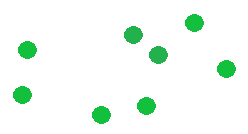
\includegraphics[width=0.5\textwidth]{./Imagenes/arista1.png}
	\caption{Eligiendo punto de inicio en azul} 
\end{figure}

\vspace{0.5cm}
\begin{figure}[htbH] 
	\centering
	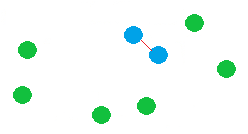
\includegraphics[width=0.5\textwidth]{./Imagenes/arista2.png}
	\caption{Tercer vértice} 
\end{figure}

\vspace{0.5cm}
\begin{figure}[htbH] 
	\centering
	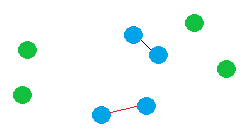
\includegraphics[width=0.5\textwidth]{./Imagenes/arista3.png}
	\caption{Cuarto vértice} 
\end{figure}

\vspace{0.5cm}
\begin{figure}[htbH] 
	\centering
	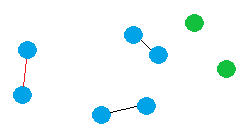
\includegraphics[width=0.5\textwidth]{./Imagenes/arista4.png}
	\caption{Quinto vértice} 
\end{figure}

\vspace{0.5cm}
\begin{figure}[htbH] 
	\centering
	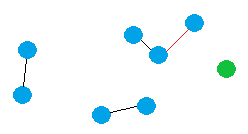
\includegraphics[width=0.5\textwidth]{./Imagenes/arista5.png}
	\caption{Sexto vértice} 
\end{figure}

\vspace{0.5cm}
\begin{figure}[htbH] 
	\centering
	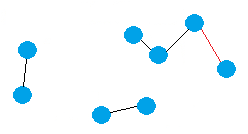
\includegraphics[width=0.5\textwidth]{./Imagenes/arista6.png}
	\caption{Séptimo vértice} 
\end{figure}


\vspace{0.5cm}

Debemos tener en cuenta que solamente podemos unir aristas que estén en dos caminos diferentes si sus puntos son extremos de caminos ya existentes. De esta forma aunque un vértice sea un extremo de un camino, si su otro extremo está en mitad de otro camino no nos vale, ya que llegaría un punto en el que pasaríamos dos veces por el mismo punto.

\begin{figure}[htbH] 
	\centering
	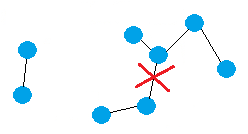
\includegraphics[width=0.5\textwidth]{./Imagenes/arista6fail.png}
	\caption{Octavo y último vértice} 
\end{figure}

\vspace{0.5cm}
\begin{figure}[htbH] 
	\centering
	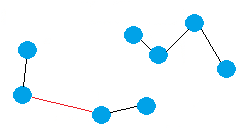
\includegraphics[width=0.5\textwidth]{./Imagenes/arista7.png}
	\caption{Octavo y último vértice} 
\end{figure}

\vspace{0.5cm}
\begin{figure}[htbH] 
	\centering
	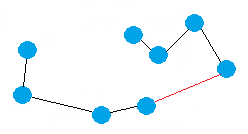
\includegraphics[width=0.5\textwidth]{./Imagenes/arista8.png}
	\caption{Octavo y último vértice} 
\end{figure}

No debemos olvidar terminar el camino.

\begin{figure}[htbH] 
	\centering
	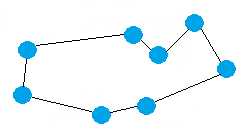
\includegraphics[width=0.5\textwidth]{./Imagenes/arista9.png}
	\caption{Recorrido vecino más cercano} 
\end{figure}

\newpage
\subsubsection{Ejemplos}
Puntos:

	\begin{figure}[htbH]
		\centering
		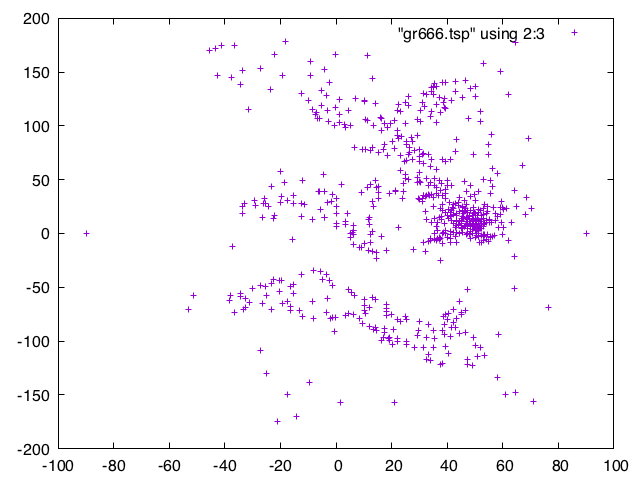
\includegraphics[width=0.65\textwidth]{../Viajante/Imagenes/gr666.png}
		\caption{Quinto vértice}
	\end{figure}
	
Recorrido óptimo:

	\begin{figure}[htbH]
		\centering
		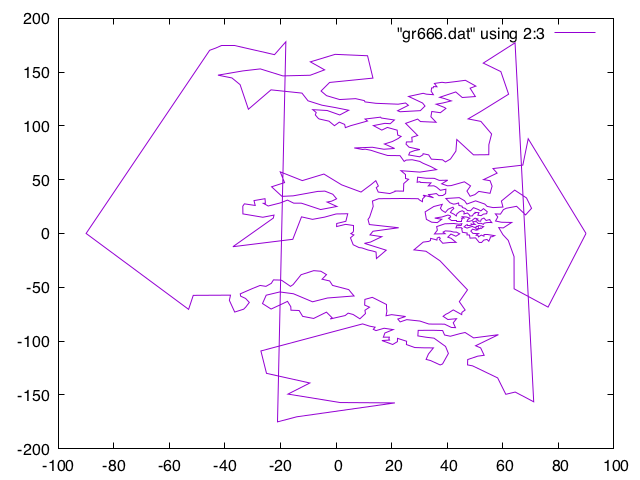
\includegraphics[width=0.65\textwidth]{../Viajante/Imagenes/gr666_opt.png}
		\caption{Quinto vértice}
	\end{figure}
\newpage

% % % % % % % % % % % % % % % % % % % % % % % % % % % % % % % % %
%					 Bibliografia
% % % % % % % % % % % % % % % % % % % % % % % % % % % % % % % % %
\section{Bibliografia}
%  https://saforas.wordpress.com/2008/01/05/codigo-c-ordenamiento-heap-sort/

\newpage

\end{document}
